\documentclass[12pt]{article}
\usepackage[babel=true]{csquotes}
\usepackage{cite}
\usepackage{epigraph}
\usepackage[toc]{glossaries}
\usepackage{tikz}
\usepackage{listings}
\usepackage{pdfpages}
\usepackage{amsthm}
\usepackage{amsmath}
\usepackage{hyperref}
\usepackage{amssymb}
\usepackage{float}
\usepackage[T1]{fontenc}

\theoremstyle{definition}
\newtheorem{definition}{Definition}[section]

\theoremstyle{definition}
\newtheorem{example}{Example}[section]

\theoremstyle{remark}
\newtheorem{remark}{Remark}[section]

\newcommand{\R}{\mathbb{R}}
\newcommand{\Q}{\mathbb{Q}}
\newcommand{\A}{\mathcal{A}}

\lstset{
    basicstyle=\ttfamily,
    columns=fullflexible,
    frame=single,
    breaklines=true,
    postbreak=\mbox{\textcolor{red}{$\hookrightarrow$}\space},
    language=Python,
    showspaces=false,
    showstringspaces=false,
    showtabs=false
}

\usetikzlibrary{calc,trees,positioning,arrows,fit,shapes,calc}

\graphicspath{{../img/}}

\newacronym{rug}{RUG}{Railster Universal Gateway}
\newacronym{fqm}{FQM}{Fleet Quality Management}
\newacronym{ui}{UI}{User Interface}
\newacronym{op}{O.P.}{Output Provider}
\newacronym{afa}{AFA}{Alternating Finite Automaton}
\newacronym{fsm}{FSM}{Finite State Machine}
\newacronym{efsm}{EFSM}{Extended Finite State Machine}
\newacronym{dfa}{DFA}{Deterministic Finite Automaton}
\newacronym{nfa}{NFA}{Non-Deterministic Finite Automaton}
\newacronym{io}{I/O}{Inputs/Outputs}
\newacronym{dtmc}{DTMC}{Discrete-Time Markov chain}
\newacronym{mdp}{MDP}{Markov decision process}
\newacronym{pa}{PA}{Probabilistic Automaton}
\newacronym{ctmc}{CTMC}{continuous-time Markov Chain}
\newacronym{pta}{PTA}{Probabilistic Timed Automaton}
\newacronym{dsl}{DSL}{Domain-specific language}
\newacronym{gpl}{GPL}{General-purpose language}
\newacronym{ta}{TA}{Timed Automata}

\newglossaryentry{railsteros}
{ name=Railster-OS,
  description={A set of sub-program running on the \gls{rug} defining the behavior of it}
}
\newglossaryentry{daemons}
{ name=daemons,
  description={Sub-programs running inside \gls{railsteros} adding functionalities to it}
}
\makeglossaries

\begin{document}

%\title{Practical case of Black-box driven verification}
%\author{Thomas Van Gysegem}
%\date\today
%\maketitle


\includepdf[pages={1}]{template.pdf}

\section*{abstract}

This thesis will describe a practical case of software testing and explain all the choices that where made during the implementation process. It will also try to provide some generic way of doing the same for a different use case given a similar running environment and constraints.

\clearpage
\pagebreak
\hspace{0pt}
\vfill
\epigraph{Program testing can be a very effective way to show the presence of bugs, but it is hopelessly inadequate for showing their absence}{Edsger W. Dijkstra , The Humble Programmer (1972)}
\vfill
\hspace{0pt}
\pagebreak

\clearpage

\tableofcontents

\clearpage

\section{Introduction}

Nowadays, software is everywhere. In banks, cars, vending machines, airplanes, televisions, ... You are using software in your everyday life even without knowing it and when you do, you expect it to meet some expectation, you don't want your plane to crash because of a software failure or a vending machine stealing your money. That's why some guidelines and processes exists to build those softwares. Those processes can last for days, months or even years before producing the expected software and during this process, some errors can be made that makes the software faulty or broken. That's why, all along this process, we need to make sure that everything is working just fine. To do that, we introduce a step in the development process called "testing". Without it, no complicated software will be able to do its task without problems. Of course, this testing step can be done differently depending on the overall development process but nevertheless, every software need to go through that step.\\

This thesis is all about this particular testing step. The goal of it will be to provide a way of automating this step. As we will explain later on, providing this automatic process is of major interest in term of time gained in the development process and reliability for the final software. Of course, detecting all problems during testing is a really complex task and the process developed throughout this thesis will only help to reduce the risk of shipping faulty softwares and to make sure that previously encountered/corrected problems are not re-introduced between different versions of it.\\

To guide us during this work, we will focus on a concrete case study that was encountered at the Railnova company in Brussels. Of course, as the goal of this work is to stay generic, we will go from the concrete examples solution to more generic solutions that can easily be extended for any other software. Despite the fact that this thesis will try to stay generic, we will not talk about hardware testing even if we can see that as a particular case of testing in a development process. We think that focusing on software development will help the reader to get a better understanding of the principles used and developed ideas.\\

I divided this work in many blocs that introduces them-self one after the other. As this topic and all the techniques involved are closely related, there will often be references to area not already covered during the sequential reading of this thesis:
First, the preliminaries will show why this work was started and what is the need that it satisfies. Then, we'll introduce software testing. We'll try to give an overview of all the main techniques and good practices currently used. After that, we will introduce the main tool we used to complete the task at hand, the \gls{fsm}. We will also give various alterations of \gls{fsm} which are relevant in our case. Then, we will introduce the context in which this work was done, where and why we had to solve such a task. Following this, we will show how we used all the previous chapters concepts to devellop our solution, what was used or not in the previously coverred topics and how we used them all together. Lastly, we will present the final product that was developed. Showing how it works and what it can do.


%------------------------------------------------------------------------%
%                                                                        %
%                                                                        %
% PRELIMINARIES                                                          %
%                                                                        %
%                                                                        %
%------------------------------------------------------------------------%

\clearpage
\part{Preliminaries}

In the following chapters, we will try to explain why software testing is an important task in any IT related buisness. We give some example of problems that can be solved using the product, Nursery, that was developped in this thesis.


%-----------------------------------------------------------------------------

\section{The economics of software testing}

%-----------------------------------------------------------------------------

Usually, when you work on a development project, you have many different development stages. The main ones are the proper development of the product and the final stage of the product, when it is shipped to the production environment.\\

Shipping the product to production simply means that you put the product into its real environment. In other words, you begin to manipulates real world data and not the tests sets that you where probably using during the development. In our case, we install a RUG running \gls{railsteros} in some engine.\\

But if the shipped product contains faults, it will probably begins to produce incorrect results and, depending on the product, it can even harm people or destroy things by using them incorrectly. The client will not be able to use the product he paid for to its full capabilities and will maybe want to switch to another company that produce more reliable products. Its easy to imagine other cases in which having fault in the final product must imperatively be avoided.\\

All of this comes with a cost, for example, we can imagine that we are working on a assembly line controller. If our controller (product) does not work correctly, the assembly line can be damaged because of incorrect usage or the materials being manipulated can be damaged too resulting in repair cost for the assembly line and incorrect/damaged product assembled that cannot be sold afterwards.\\

In the \gls{rug} ecosystem, if our product, \gls{railsteros} isn't working well, the \gls{rug} its running on will not send the intended data to the client. For him, it is like the engine itself is malfunctioning or not functioning at all if we are unable to send any data! He will then need to send a team to the engine to find the problems and a lot of work will be delayed because the engine is not running and, of course, every step in this process is very costly for the client and for the company itself because when a product in production is faulty, we also need to get back the devices that are malfunctioning and, perhaps, every other device running the same software of having the same hardware. And finally, we need to replace them and invest time in correcting them or, at least, solving the issue for the other product versions.\\

\begin{figure}
    \centering
    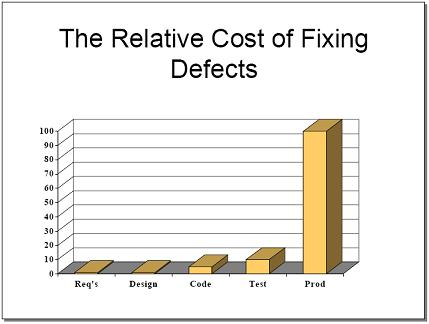
\includegraphics[scale=0.8]{STBC-costfixs.jpg}
    \caption{Relative costs of fixing faults~\cite{EconomicsSTBC:2017}}
    \label{STBC-costfixs}
\end{figure}

It is commonly believed that the earliest a fault is found, the cheaper it is to correct it~\cite{EconomicsSTBC:2017}~\cite{EconomicsWiki:2017}. The case we mentioned is the latest possible time to detect a fault so, according to the previous statement, it is also the most expensive! Those reasons are why we want to create some process that can be used to drastically reduces the amount of unexpected faults in the final product. That's the main motivation behind the project that is the subject of this thesis called Nursery.\\


%-----------------------------------------------------------------------------

\section{Our case}
\label{section:ourcase}

%-----------------------------------------------------------------------------

%// TODO concrete case here

%-----------------------------------------------------------------------------

\section{Related works}

%-----------------------------------------------------------------------------

%// TODO Related works
%Chow:1978:TSD:1313335.1313730
%10.1007/978-3-540-39929-2_3

%-----------------------------------------------------------------------------

\section{Conclusion}

%-----------------------------------------------------------------------------

We have explained briefly what is the final product expected from this thesis. Keeping that in mind should help you to understand the following chapters and the reasons why we need to talk about software development and finite state machine.


%------------------------------------------------------------------------%
%                                                                        %
%                                                                        %
% SOFTWARE TESTING                                                       %
%                                                                        %
%                                                                        %
%------------------------------------------------------------------------%


\clearpage
\part{Software development and software testing}

Software development is a complex area and different processes exists but at the very last, they all have some key principles in common. One of them being the testing part. For this work to be fully understood, we need to introduce a bit of software development and then, explain which are the different techniques used in software testing. This will provide us with the required technical vocabulary to describe our own testing process.

Software development can be defined in different ways, every one of them being more or less equivalent but in this work, we will focus on the basis and simply say that software development is some kind of plan to produce a given software. This plan can be more or less complex and must involves at some point, some testing steps.\\

Software is usually ordered by a client that can be ourself, some company or any set of users~\cite{SoftwareDevelopment:2016}. Clients have needs and our task as software developer will be to fulfill them by producing a software. The client's request will first be translated into requirements specifications that, to put it simply, are formal description of them. We usually create those requirements specifications during meetings with the client, this requires meetings and discussions to be sure that the idea we get from them is what they want.\\

Then the software can be built. Of course, if we got the wrong requirements specifications, our software will not be what the client asked and therefore, they will want us to fix that and updates the requirements but modified requirements can invalidate the choosen architecture or software decisions thus requiring in depth mmodification of the current built product. Let's assume that those requirements are good, then, once the software is built, we want to test it to ensure that it works and that it meets the given requirements. Once those test are successfully passed, we can ship the software to our client.\\

This whole process, starting from the client order to the shipping of the produced software is what we call the software development process. Of course, there is not one only way of doing it even for the most simple process like this one their can be divergence of work-flow from one team to another.~\cite{IIS2:IIS202348} The goal here is to show that testing is crucial wathever the choosen methodology or software development process, we will now introduce three of them that we think are the most used or accessible for neophytes:

\begin{itemize}

\item Waterfall
\item Prototyping
\item Design: resulting in the software architecture
\item Coding: the development, proving, and integration of software
\item Testing: the systematic discovery and debugging of defects
\item Operations: the installation, migration, support, and maintenance of complete systems

\end{itemize}


\clearpage


%-----------------------------------------------------------------------------

\section{Waterfall}

%-----------------------------------------------------------------------------

The waterfall model is probably the most basic development process still used today, it is often attributed to Winston Walker Royce in a paper from 1970~\cite{BARYWBoehm:1987}. The whole process is sequential or plan driven. The whole process is divided in big parts and each of them is done only one time and one after the other. The original model was designed as follows:\\

\begin{itemize}

\item System and software requirements: captured in a product requirements document
\item Analysis: resulting in models, schema, and business rules
\item Design: resulting in the software architecture
\item Coding: the development, proving, and integration of software
\item Testing: the systematic discovery and debugging of defects
\item Operations: the installation, migration, support, and maintenance of complete systems

\end{itemize}

The following problems can easilly be spotted in this process:

\begin{itemize}

\item If an error is made during the analysis step, this error is repercuted to the next steps.
\item Between the first and the last step of it, there can be a lot of weeks, months or years! During this time, the project needs can evolve and then, the delivered product will only match outdated requirements, which, of course, is not a good thing for the client.
\item If some problems occurs during the writing of the product requirements, let's say that the client forget to talk about a key feature. Then, again, the product we will deliver will miss that feature.

\end{itemize}

Probability to produce the wrong product is high because of those problems and because of that, organizations/teams tends to avoid it when possible. Nevertheless, there is still advantages to use this process. As the first steps are strongly related to documentation of the product, if a team member leaves during the process, we have less risk of loosing knowledge of what has been done or what is left to do. New team members will simply need to read the requirements, the produced models and the software architecture.\\

This process is also one of the easiest to understand, every step of the project is well documented and one can easily jump in any project using this methodology and be ready to participate in a very short time.\\

\begin{figure}
    \centering
    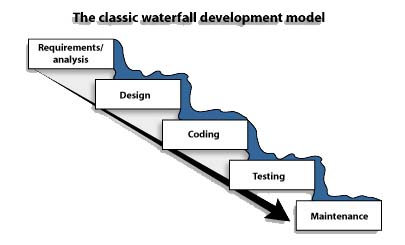
\includegraphics[scale=0.8]{waterfall.jpg}
    \caption{Waterfall model. You should see why it is called waterfall from this picture.}
    \label{Waterfall}
\end{figure}


%-----------------------------------------------------------------------------

\section{Prototyping}

%-----------------------------------------------------------------------------

Sometimes, you want to produce a product as soon as possible so you can conquer the market sooner. In that case, the waterfall approach is not going to be very useful. The prototyping process though, can help you towards this goal.~\cite{Software_prototyping:2018}\\

The idea is to produce some prototype as soon as possible, test it and then, iterate over it again and again until the final product is fully functional. It is a trial-and-error process. This works especially well when the final product requirements are not fully known. By presenting a prototype to the client, he is able to give feedbacks and explain the following most wanted features. Like for the waterfall model, we have a plan for the whole process: The whole product is divided into as many sub-product as needed. Each of those division will be prototyped on top of the last ones until we get the final product.\\

\begin{itemize}

\item System requirements are defined in as much details as possible.
\item A first design is created.
\item The first prototype is created.
\item Client tests/reviews the prototype.
\item Developers change the prototype accordingly.
\item We repeat those steps as many times as needed.
\item The final product is constructed based on the last prototype.

\end{itemize}

Using this model, the probability to deliver a product that does not meet the client requirements is very small as he can give a feedback throughout the whole development process. But there are some drawbacks to that.\\

Focusing on small sub-problems/sub-features distracts the developers from conducting a good and in depth analysis. This is also due to the lack of fully specified requirements from the start. Adding more and more features on top of existing ones can quickly create a complicated product both difficult to maintain and improve.\\

\begin{figure}
    \centering
    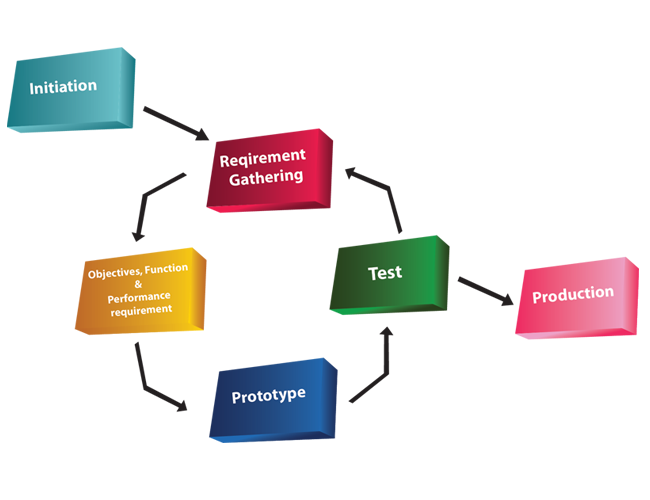
\includegraphics[scale=0.4]{prototyping.png}
    \caption{Schema of the prototyping process.}
    \label{Prototyping}
\end{figure}


%-----------------------------------------------------------------------------

\section{Agile}

%-----------------------------------------------------------------------------

Agile Software Development is based on twelve principles:~\cite{agile_manifesto:2018}

\begin{itemize}
\item Customer satisfaction by early and continuous delivery of valuable software
\item Welcome changing requirements, even in late development
\item Working software is delivered frequently (weeks rather than months)
\item Close, daily cooperation between business people and developers
\item Projects are built around motivated individuals, who should be trusted
\item Face-to-face conversation is the best form of communication (co-location)
\item Working software is the principal measure of progress
\item Sustainable development, able to maintain a constant pace
\item Continuous attention to technical excellence and good design
\item Simplicity or the art of maximizing the amount of work not done is essential
\item Best architectures, requirements, and designs emerge from self-organizing teams
\item The team reflects on how to become more effective, and adjusts accordingly
\end{itemize}

There exist many different frameworks that complies to those principles. One of the most commonly used is Scrum~\cite{ScrumAlliance:2017}~\ref{Scrum}. With this framework, we work using sprints. A sprint is the basic unit of development in Scrum. The team fixes the time-frame during which the sprint must be done and then, fixes the scope of work that needs to be done during a Sprint Planning event.\\

At the end of each day, the team holds a Daily Scrum to answer the following questions:

\begin{itemize}
\item What did I do?
\item What will I do to meet the sprint goals?
\item Is there anything that block the team progress?
\end{itemize}

Finally, at the end of the sprint period, the team holds a Sprint Retrospective to answer the following questions:

\begin{itemize}
\item What went well?
\item What could be improved?
\end{itemize}

This allows for a very dynamic development process in which no one gets stuck too long on ineffective or impossible processes.

\begin{figure}
    \centering
    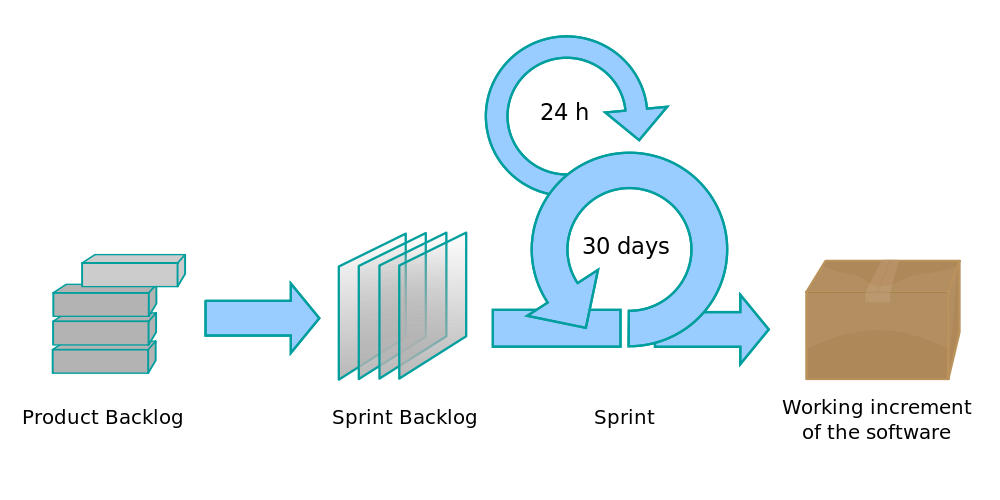
\includegraphics[scale=0.4]{scrum.png}
    \caption{Schema of the Scrum Framework. A popular development process. This is only an example, the sprint duration is not always 30 days.}
    \label{Scrum}
\end{figure}


%-----------------------------------------------------------------------------

\section{Validation and verification}

%-----------------------------------------------------------------------------

Now that we have settled down our requirements specifications, we need to introduces the validation and verification topic. Validation and verification is what we use to make sure that our software is meeting the previously specified requirements. In short, that our software is exactly what we specified. Failing to this would produce a software that will maybe not meet the clients requirements and, therefore, be of little or no use to him.\\

Both concepts are closely related but are completely independent. Software validation is a procedure used to ensure that the software meets the user's needs and that the specifications were correct while software verification is a procedure used to ensure that the software follows the specified requirements~\cite{VnV:2016}. Following is a more formal definition:

\begin{itemize}

\item \textbf{Validation} is the confirmation by examination and through provision of objective evidence that the requirements for a specific intended use or application have been fulfilled~\cite{IEEEStd1990}
\item \textbf{Verification} is the confirmation by examination and through provision of objective evidence that specified requirements have been fulfilled~\cite{IEEEStd1990}

\end{itemize}

Simply put, validation is answering to \guillemotleft Are we trying to build the right thing?\guillemotright while verification is answering to \guillemotleft Have we made what we were trying to make?\guillemotright. Of course, in our case, we are more interested in the verification part and we will leave the validation part out of this work. We will assume that the requirements are correct and therefore that if we follow them, the built software will be the one our client wants.


%-----------------------------------------------------------------------------

\section{Code coverage}

%-----------------------------------------------------------------------------

Code coverage is a metrics used in software testing that basically tells you how much of your code has been tested. It can be computed on many different criteria like how many subroutines have been called, how many lines of code have been interpreted and so on.\\

The idea behind this metric usage is that, if all of your code is tested, then there is probably no bugs left, or at least, there is a good probability that we will encounter fewer bugs in a completely tested software than in an untested one. Getting a good code coverage is therefore a key point in testing as it improve the software quality by reducing the probability of faults left in it~\cite{TestingForContinuousDelivery:2016}.\\

You can compute code coverage differently based on the testing requirements. Here is a non exhustive list of some criteria you can use to compute it:

\begin{itemize}
\item \textbf{Function coverage} Percentage of defined functions called during testing.
\item \textbf{Statement coverage} Percentage of statements called during testing.
\item \textbf{Branch coverage} Percentage of branching possibility executed during testing.
\end{itemize}

Using one or several code coverage criteria, you can define a threshold used to certify that the product is unlikely to contains fault. For example, you can requires that 95\% of defined functions are called during tests.


%-----------------------------------------------------------------------------

\section{Black-box and white-box testing}

%-----------------------------------------------------------------------------

Black-box testing and white-box are two terms used by softwares testers to describe how they approach their testing~\cite{Patton:2005}. They describe two of the most common used techniques in software testing.

With black-box testing, also known as functional testing, we consider the software as a black-box and we have no knowledge of what is inside of it nor on how it works. This is the opposite of white-box testing where the whole software is known from the inside, all the code is accessible and we have a deep knowledge of how it works.\\

Both of those approaches have their own advantages and drawbacks. In white-box testing, the tester is testing functionalities that are already developed and he can miss needed features that have been forgotten. He has a very good code coverage as he can produce test cases for every specific details by reading the code. White-box provides an internal perspective of the software.\\

Black-box testing, on the other hand, provides another point-of-view and does not require a deep knowledge of the code to operate. Test cases are designed following the requirements and not the code itself so if all the tests are successful and that all the requirements are entirely covered by the designed test, we have a proof that our software meets the requirements.\\

White-box testing is more or less done by developers themselves while black-box testing can be performed by anyone with poor programing skills. Code coverage can not be used while doing black-box testing for the obvious reason that you don't know what is done internally so you don't know what part of the software code is interpreted.


\subsection{Grey-box testing}
%-----------------------------------------------------------------------------

There is also a third option there which is called \guillemotleft Grey-Box testing \guillemotright . We are doing Grey-Box testing when we do both Black-Box testing and White-Box testing. In Black-box testing, you don't have knowledges of the internal structure of code while in White-box testing, you do have this knowledges. Grey-box testing is when you do have a limited knowledge of the internal structure of code. You can get an idea of this with the following scenario: Let's say we want to check a sign-in feature for a service where you have a client software and a server that provides the service. If you have access to the source code for the client software, testing the sign-in feature using this knowledge is called Grey-box testing as you only have limited knowledge of the underlying structure of code.


%-----------------------------------------------------------------------------

\section{Static and Dynamic testing}

%-----------------------------------------------------------------------------

Two other terms used in software testing are static and dynamic testing. Static testing is the process of reviewing something that is not running. For example, some compilers (like gcc) perform static testing by finding unaffected variables, unused variables, dead code, syntax errors and so on. Dynamic testing, on the other hand, is performed while the program is running~\cite{StaticDynamicTesting:2018}.


%-----------------------------------------------------------------------------

\section{Type of testing}

%-----------------------------------------------------------------------------

There exists a lot of different types of software testing, explaining them all is way out of the boundaries of this work so we have chosen 6 of them that are closely related and can be spanned on a whole software development process~\cite{Laurie.W:Black-box}.


\subsection{Unit testing}
%-----------------------------------------------------------------------------

Scope: White-box testing\\
Who: Coder\\

Unit testing is a software testing method by which individual units of source code, sets of one or more computer program modules together with associated control data, usage procedures, and operating procedures, are tested to determine whether they are fit for use. The goal is to isolate each part of the program and show that the individual parts are correct~\cite{AutomatedDefectPrevention:2007}.\\

In a more practical point-of-view, it's about isolating each function or method in the code and test their behavior for a wide range of input values. A lot of faults can stay undetected after this step. One of the reason of this being that people who write unit-test have a deep knowledge of the underlying code. This knowledge introduces biases and influences them when writing unit-test so it is easy to miss use cases because the programmer assume unconsciously that they are working. Also, if those who write the unit-test are the same ones that wrote the code that is being tested, the test code is likely to be as faulty as the code being tested itself!

\begin{figure}
\label{unit_testing_sample}
\begin{lstlisting}[caption=Brief example of what unit testing is (C pseudocode),label={lst:unit_testing_sample}]
/**
 * @brief Reads a file content
 * @param name Name of the file
 * @param buffer Buffer for the file content
 * @return 0 and buffer is filled with the file content.
 *         -1 if file does not exists
 *         -2 if file can't be read
 */
int readFile(const char* name, const char* buffer);

// Tests fake file name
assert(readFile("doesnotexist.txt", buffer) == -1);

// Tests file can't be read
assert(readFile("busyFile.txt", buffer) == -2);

// Tests file read success
writeFile("file.txt", "some text");
assert(readFile("file.txt", buffer) == 0);
assert(buffer == "some text");
\end{lstlisting}
\end{figure}


\subsection{Integration testing}
%-----------------------------------------------------------------------------

Scope: Black-box and white-box testing\\
Who: Coder\\

Integration testing is the phase in software testing in which individual software modules are combined and tested as a group. It occurs after unit testing and before validation testing. Integration testing takes as its input modules that have been unit tested, groups them in larger aggregates, applies tests defined in an integration test plan to those aggregates, and delivers as its output the integrated system ready for system testing~\cite{TestingInSoftwareDevelopment:1987}.\\

A good example for this would be a serial communication library. You have a module with several basic functions/blocs for serial devices manipulation like:
\begin{enumerate}
\item Sending a byte over a serial port
\item Receiving a byte using the serial port
\item Openning a serial port
\item Closing a serial port
\end{enumerate}

An integration test could be done by checking by having a device that sends data through the serial port an expects the same data as a result. In this example you would have to use all the basic blocs that determines the module features.


\subsection{Functional testing}
%-----------------------------------------------------------------------------

Scope: Black-box testing\\
Who: Independent tester\\

Functional testing is about testing each functionality of the whole system as described in the requirements.

Functional testing tests a slice of functionality of the whole system. Functional testing does not imply that you are testing a function/method of your module or class. If the functionalities wanted are:
\begin{enumerate}
\item Sending invoices to clients
\item Creating invoices
\item Adding clients
\end{enumerate}

Then you will have test cases that try to add clients, another one that try to send invoices and acknowledges that the client, preferably a fake one, received it and a last test case that will create various different invoices.


\subsection{System testing}
%-----------------------------------------------------------------------------

Scope: Black-box testing\\
Who: Independent tester\\

System testing involves putting the new program in many different environments to ensure the program works in typical customer environments with various versions and types of operating systems and/or applications~\cite{Laurie.W:Black-box}. System testing is testing conducted on a complete, integrated system to evaluate the system compliance with its specified requirements~\cite{IEEEStd1990}.\\

This is very relevant in computer science where every computer is built from different component and can have many different operating systems. To perform system testing, you will usually run the program on different operating systems (Unix based systems or DOS based systems) and also on different hardware configuration. Of course, testing every possible combination is not possible so some exotic systems can still prove themselves unable to run the program after this steps. Of course, if your program is built to run on a specific pre-defined system, this testing will be really straightforward.

A basic example of system testing would be two computer, one running a Unix based operating system and the other running Windows for example (any version will do). In this case, the system test would be to run the program in both environment (Unix based OS and Windows) and check that, given the same inputs, both of them produces the same results or at least, similar enough ones. In other words, verify that they both works as expected.


\subsection{Acceptance testing}
%-----------------------------------------------------------------------------

Scope: Black-box testing\\
Who: Client\\

Acceptance testing is formal testing conducted to determine whether or not a system satisfies its acceptance criteria (the criteria the system must satisfy to be accepted by a customer) and to enable the customer to determine whether or not to accept the system. More formally, the system is tested to verify that it meets the given specifications or contract.\\

Usually, the user will provide some test or use case for each desired functionality. You can add your own test to those but at least the client test must be satisfied before trying to deploy the product otherwise the client will probably not even try the product.


\subsection{Regression testing}
%-----------------------------------------------------------------------------

Scope: Black-box and white-box testing\\
Who: Coder\\

Regression testing is a type of software testing used to ensure that a software that was previously developed and tested still meets the previously defined requirements after a modification has been introduced into it such as a bug fixes or enhancements. The purpose is to make sure that the newly introduced modifications do not damage any previously-working functionality.\\

Practically speaking, we will only add new test when we are adding new functionalities and we will remove test only when the functionality covered is no longer needed or maintained. Then, if all the tests are still running without error on our new software, we will assume that previously developed functionality still works.


\subsection{Beta testing}
%-----------------------------------------------------------------------------

Scope: Black-box testing\\
Who: Client\\

This step is performed when the software is fully or well developed. The software is shipped to a limited amount of users so that they can test it as they wish. The purpose is to detect fault by providing inputs that testers have not thought about because of their advanced knowledge of the software and its purpose.


%-----------------------------------------------------------------------------

\section{Requirements-based testing}

%-----------------------------------------------------------------------------

Requirements-based testing is a testing approach in which test cases, conditions and data are derived from requirements~\cite{IBMRequirementBasedTesting:2017}. Those test can be performed from the start of the development process and to the end of it~\cite{BenderRBTRequirementBasedTesting:2017}. Of course, if the requirements are not good, those test will be of little use. Good requirements are critical but requirements checking is, again, out of our scope. So we will simply assume that we have good requirements for this work.\\

Requirements-based testing is exactly what we are trying to do with black-box testing. For each given requirements stating, for example, that we want to produce some result Y when you give some input X, we want to produce a test case that maps the input X to our software and gets the output Y'. Comparing Y and Y' will allow us to decide whether or not, there is a fault and/or decide if the requirement is met or not. If not, our software is not built correctly and we need to work more on it before shipping it for the client.\\

All the previously described type of testing are not necessarily requirements-based. For example, unit testing is about the code. We want to make sure that each part of the code work well but satisfying that does not imply that requirements are met! For a 3D modeling software, we can have a code that compute square roots, if the code works well, that does not imply that our software allows the user to design houses for example.\\


%-----------------------------------------------------------------------------

\section{Conclusion}

%-----------------------------------------------------------------------------

You should now have a good idea of why testing is of crucial importance in any software development process as well as some pointers on what needs to be tested, validated and verified all along the development process. Given requierments, the software development process should produce a software that meet those requirements. Let's now introduce the core aspect of this thesis, model checking.


%------------------------------------------------------------------------%
%                                                                        %
%                                                                        %
% MODEL CHECKING                                                         %
%                                                                        %
%                                                                        %
%------------------------------------------------------------------------%

\clearpage
\part{Formal Verification and Model Checking}\label{ModelChecking}

Our goal is to be able to verify that any kind of product, software or hardware, is working as expected. Formal verification can help us to achieve this goal. It is a process that allows us to check whether or not a given model satisfies given properties. You can, for example, create a model of a given software and verify that it does not contain bugs. To be able to do that, both the model and the specification must be formally described in a mathematical language. The model is an abstraction of the real system which can have some properties. The requirements we want to check must be expressed as properties which can then be checked against the model using \gls{fsm} that we will now introduce.\\


\clearpage


%-----------------------------------------------------------------------------

\section{Finite State Machine}

%-----------------------------------------------------------------------------

An \gls{fsm} is a mathematical model of computation. It is a mathematical structure used to provide an abstract description of the behavior of a system. This mathematical structure is composed of a set of states. An \gls{fsm} can be in exactly one of a finite number of states at any given time. The FSM can change from one state to another in response to some external inputs. The function that maps state and inputs to states is called a transition. An FSM is defined by its set of states, its initial state, the input alphabet and a set of transitions~\cite{FSM:2017}.\\

\begin{figure}[H]
    \centering
    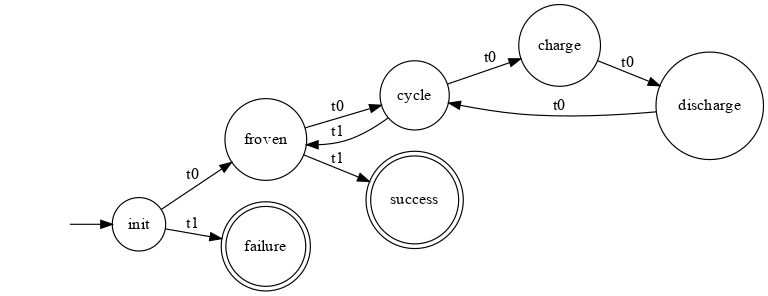
\includegraphics[scale=0.4]{graph/BatteryCycle.png}
    \caption{Example of an \gls{fsm} shown as a graph.}
    \label{battcycle}
\end{figure}

The input alphabet is the set of every symbol the \gls{fsm} can receive in any given state. For example, an input alphabet could be a list of keyboard's key if we consider an \gls{fsm} that simulates the behavior of a text editor. The key points here are that you need to have a finite set of states and a finite set of transitions.\\

\theoremstyle{definition}
\begin{definition}{Finite alphabet.} A finite alphabet $\Sigma$ is a finite set of symbols.
\end{definition}

\theoremstyle{definition}
\begin{definition}{State-transition function.} A state-transition function $\delta$ is a mapping $\delta:S\times \Sigma \rightarrow S$ that maps each state $s$ with a symbol $a$ from an input alphabet $\Sigma$ and another state $s'$.
\footnote{This hold only for deterministic \gls{fsm}, we'll see later how to express $\delta$ for non-deterministic \gls{fsm} and what non-deterministic/deterministic \gls{fsm} means.}
\end{definition}

\theoremstyle{definition}
\begin{definition}{Finite State Machine.} an \gls{fsm} is a quintuple $(\Sigma, S, s_{0},\delta, F)$, where:
\begin{itemize}
\item $\Sigma$ is the finite input alphabet.
\item $S$ is the set of states.
\item $s_{0} \in S$ is the initial state.
\item $\delta$ is the state-transition function: $\delta: S \times \Sigma \to S$.
\item $F \subseteq S$ is the set of final states.
\end{itemize}
\end{definition}

Because of those rules, a transition function can start and end in the same state, thus creating a loop on the state. $\delta$ is conventionally allowed to be a partial function. This means that $\delta(s, e)$ does not needs to be defined for every possible combination of $s \in S$ and $e \in \Sigma$. This allows us to have a finite $\delta$ transition function even when the input alphabet $\Sigma$ is not totaly known or infinite. In our case, this allows to describe a \gls{fsm} by only specifying transition function for input we are actually interested in which can be helpful if we have a huge input alphabet.\footnote{As you'll see later, we will have to describe \gls{fsm} that have a huge input alphabet, this saves us a lot of time by only requiring us to describes what happen for symbols that actually are of interest for us.}

%About the input alphabet, we usually define every input as a character or token read on the input tape of the \gls{fsm}. Where the input tape is a sequential list of every symbols feed into the system. This is a lot like a Turing Machine.

\theoremstyle{definition}
\begin{definition}{Finite word.} A finite word $\sigma = \sigma_1 \sigma_2 ... \sigma_n$ is a finite sequence of symbols from $\Sigma$: $\forall i: \sigma_i \in \Sigma$.
\end{definition}

%\theoremstyle{definition}
%\begin{definition}{Transition table.} A transition table $\A$ is a tuple $(\Sigma, S, s_{0}, \Delta)$, where:
%\begin{itemize}
%\item $\Sigma$ is the input alphabet.
%\item $S$ is the set of state.
%\item $s_{0} \in S$ is the initial state.
%\item $\Delta \subseteq S \times S \times \Sigma$ is the set of state-transitions function.
%\end{itemize}
%\end{definition}

A \gls{fsm} can be run over a finite word from the input alphabet in order to accept or reject it. This is formally defined as follows:

\theoremstyle{definition}
\begin{definition}{Run.} A run $r$ of the \gls{fsm} $\A = (\Sigma, S, s_{0}, \Delta, F)$ over a finite word $\sigma = \sigma_1 \sigma_2 ... \sigma_n$ over the alphabet $\Sigma$ is a sequence of states and alphabet symbols
$$r: \overline{s} = s_0 \xrightarrow[]{\sigma_1} s_1 \xrightarrow[]{\sigma_2} s_2 \xrightarrow[]{\sigma_3} ... \xrightarrow[]{\sigma_n} s_{n+1}$$ where $\forall i \ge 1: (s_{i-1}, s_i, \sigma_i) \in \Delta$
\end{definition}

\theoremstyle{definition}
\begin{definition}{Accepting run.} A run $r$ of the \gls{fsm} $\A = (\Sigma, S, s_{0}, \Delta, F)$ over a finite word $\sigma = \sigma_1 \sigma_2 ... \sigma_n$ over the alphabet $\Sigma$ is an accepting run if:
$$s_{n+1} \in F$$
$$r: s_0 \xrightarrow[]{\sigma_1} s_1 \xrightarrow[]{\sigma_2} s_2 \xrightarrow[]{\sigma_3} ... \xrightarrow[]{\sigma_n} s_{n+1}$$ where $\forall i \ge 1: (s_{i-1}, s_i, \sigma_i) \in \Delta$
\end{definition}

\theoremstyle{definition}
\begin{definition}{Rejecting run.} A run $r$ is a rejecting run if it is not an accepting run.
\end{definition}

We can extend the definition of \gls{fsm} by splitting the final states in two distinct set: success states and failure states.

\theoremstyle{definition}
\begin{definition}{(Extended) Finite State Machine.} A \gls{efsm} is a tuple $(\Sigma, S, s_{0},\delta, W, F)$, where:
\begin{itemize}
\item $\Sigma$ is the finite input alphabet.
\item $S$ is the set of state.
\item $s_{0} \in S$ is the initial state.
\item $\delta$ is the state-transition function.
\item $W \subseteq S$ is the set of final success states.
\item $F \subseteq S \\ W$ is the set of final failure states.
\end{itemize}
\end{definition}

This extension of finite state machine doesn't introduce any more complexity. Take the original definition where a finite state machine FSM is a tuple $(\Sigma, S, s_{0},\delta, A)$. In this definition, the set of final state $A$ is equivalent to $W \cup F$ from our extended definition.

With this new defintion in mind, we define a run to be a \textit{successful run} and \textit{failed run}: Every run is a said to fail if it is not a successful run. Now, we define a successful run as a run where at least one state is a success state and no previous state is a failure state:

\theoremstyle{definition}
\begin{definition}{Successful run.} A run $r$ of the \gls{efsm} $\A = (\Sigma, S, s_{0}, \Delta, W, F)$ over a finite word $\sigma = \sigma_1 \sigma_2 ... \sigma_n$ over the alphabet $\Sigma$ is a successful run if:
$$\exists s_i \in \overline{s} | s_{i} \in W$$ and $$\forall j < i: s_{j} \notin F$$
\end{definition}

\theoremstyle{definition}
\begin{definition}{Failure run.} A run $r$ of the \gls{efsm} $\A = (\Sigma, S, s_{0}, \Delta, W, F)$ over a finite word $\sigma = \sigma_1 \sigma_2 ... \sigma_n$ over the alphabet $\Sigma$ is a failure run if it is not a successful run.
\end{definition}

%To determine what is a successful run, assume at least one state $s_i$ from $r$ is in $W$: Take the one with the smallest $i$. If $i$ equals $0$, the run is accepting, if not: if $\forall j < i: s_j \notin L$ then its an accepting run.


\subsection{Description of Finite State Machine using graphs}
%-----------------------------------------------------------------------------

Having a more human friendly way of presenting \gls{efsm} is possible using graphs. To show an \gls{efsm} as a graph, we use a directed empty graph $G$. Then, we create a node for every state of our \gls{efsm}. Now we add an edge for every transition defined in $\delta$ with the starting point being the current node and the endpoint is the node corresponding to the goal of the transition. Finally, we add an edge starting from nowhere and pointing to the node representing the initial state.\\

Every state $s$ in $W$ or $F$ is displayed with a double circle. We label those in $W$ with "\textit{success}" and those in $F$ with "\textit{failure}". This gives us a graph we can display like in the Figure~\ref{battcycle}. For comprehension sake, we have also labeled each node with a brief state name and every transition with an unique name based on the starting node.


%-----------------------------------------------------------------------------

\section{Acceptors}

%-----------------------------------------------------------------------------

An acceptor takes a sequence of inputs from the input alphabet and runs an \gls{fsm} on it. Every state of the acceptor is either and accept state or a reject state. When the computation ends in an accepting state, we say that the input is accepted and the input is not accepted otherwise (Figure~\ref{acceptor}). The set of sequence of input symbols accepted by an acceptor is called a regular language.

\begin{figure}
    \centering
    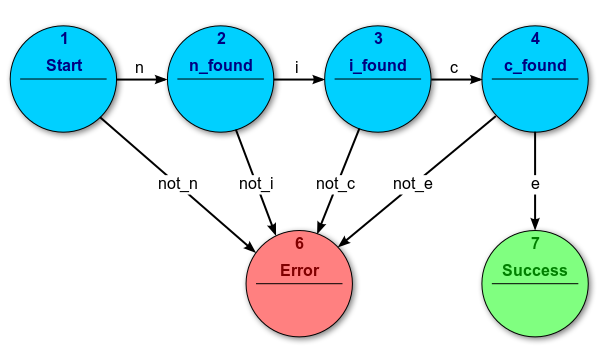
\includegraphics[scale=0.8]{acceptor.png}
    \caption{Example of acceptor for the string 'nice'~\cite{FSM:2017}}
    \label{acceptor}
\end{figure}


%-----------------------------------------------------------------------------

\section{Language}

%-----------------------------------------------------------------------------

We define a word over a given alphabet as a sequence of symbols from that alphabet. As you already know, a \gls{fsm} is defined for an input alphabet and all sequence of symbols from that alphabet are words. We also define a language as a set of words.

\theoremstyle{definition}
\begin{definition}{Language.} A language $L$ over an alphabet $\Sigma$ is a subset of $\Sigma^*$, a set of word over the alphabet.
\end{definition}

An \gls{fsm} can accept or reject words, we will call the set of accepted words a regular language over the input alphabet of the \gls{fsm}.

\theoremstyle{definition}
\begin{definition}{Regular Language.} A language $L \subseteq \Sigma*$ is regular if all word $w \in L$ are accepted by an \gls{fsm} $A$.~\cite{Yu:1997:RL:267846.267848}
\end{definition}

We define the language recognized by an \gls{efsm} as follows:
\theoremstyle{definition}
\begin{definition}{Language of an \gls{efsm}.} The language $L \subseteq \Sigma*$ recognized by an \gls{efsm} is the set of all words that produce successful run for the \gls{efsm}.
\end{definition}


%-----------------------------------------------------------------------------

\section{Non-Determinism}

%-----------------------------------------------------------------------------

A \gls{nfa} is a kind of \gls{fsm} in which transitions do not requires the reading of input symbols. We can take transitions from one state to another without looking at the input tape. The decision of taking such a transition is done in a non-deterministic way and there can be several transition that are valid from the same state for the same input symbols. For example, in the Figure~\ref{nfa}, reading symbol $1$ while in state $p$ can give two outcomes: either we go in state $q$ or we stay in state $p$.~\cite{FA-DecisionProblems:1959}

Formally speaking, we represent a \gls{nfa} with a 5-tuple, $(Q, \Sigma, \Delta, q_0, F)$ where:

\begin{itemize}
\item $Q$ is the finite set of states.
\item $\Sigma$ is the input alphabet.
\item $\Delta$ is the transition-function $\Delta: Q \times \Sigma \rightarrow P(Q)$ where $P(Q)$ is the power-set of $Q$.
\item $q_0$ is the initial state with $q_0 \in Q$.
\item $F$ is the set of accepting states where $F \subseteq Q$.
\end{itemize}

In an \gls{nfa}, the input alphabet $\Sigma$ usually contains a special symbol for representing a transition that can be taken without reading the next input symbol on the tape. This symbol is $\epsilon$.\\

\begin{figure}
    \centering
    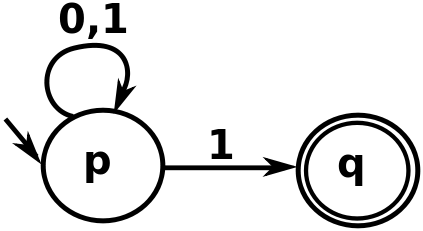
\includegraphics[scale=0.4]{graph/nfa.png}
    \caption{Example of a \gls{nfa}. In state $p$, reading the symbol $1$ can lead to $p$ or $q$~\cite{NFA:2017}}
    \label{nfa}
\end{figure}

A run of a \gls{nfa} produces several set of transitions instead of only one like it did for a \gls{fsm}. From this, we say a run is accepting if when the last input symbol is consumed, there is at least one of the produced set of transition that ends in an accepting state. Similarly, we define a rejecting run as a run that do not produce a sequence of transition that ends in an accepting state.\\

It is known that we can construct an equivalent \gls{dfa} from a \gls{nfa} and they recognizes the same language.~\cite{10.1007/3-540-63174-7_12}


%-----------------------------------------------------------------------------

\section{Alternating Finite Automaton}

%-----------------------------------------------------------------------------

An \gls{afa} is a 6-tuple, $(S(\exists), S(\forall), \Sigma, \delta, P_0, F)$, where:

\begin{itemize}
\item $S(\exists)$ is a finite set of existential states
\item $S(\forall)$ is a finite set of universal states
\item $\Sigma$ is a finite set of input symbols
\item $\delta$ is a state-transition function $\delta: (S(\exists) \cup S(\forall)) \times (\Sigma \cup \{ \epsilon \}) \rightarrow 2^{S(\exists) \cup S(\forall)}$
\item $P_0$ is the initial state with $P_0 \in (S(\exists) \cup S(\forall))$
\item $F$ is the set of final state with $F \subseteq (S(\exists) \cup S(\forall))$
\end{itemize}

In an \gls{afa}, transition are more complex than those we encountered in traditional \gls{fsm}. The transition we are working with can lead to more than one state! This is used to represent logical AND and OR with transitions (see figure~\ref{afa}).\\

\begin{figure}
    \centering
    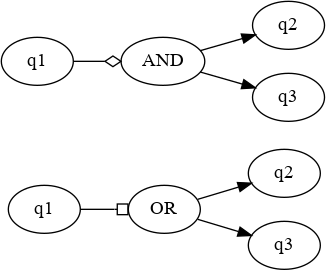
\includegraphics[scale=0.8]{graph/afa.png}
    \caption{Example of a \gls{afa}.}
    \label{afa}
\end{figure}

To implement this automaton, we need to be able to store the system's current state and restore it later so we can do multiple run and back-track when needed for every existential and universal transition we have. When we take an AND transition, we need to run a second automaton in parallel for each state the transition leads to and when we encounter an OR transition, we behave like a non-deterministic automaton by taking one of the possibilities non-deterministically. Depending on the number of those transitions, this increase the memory usage of our automaton as well as the time needed to complete the evalutation of all possible paths.\\

The computation of such an automaton is a tree. And deciding whether or not an \gls{afa} accepts a word $w$ if there exists a run tree on $w$ such that every path ends in an accepting state.~\cite{AFA:2017}\\

%\subsection{Markov model}
%
%Markov Model is a stochastic model used to model randomly changing systems~\cite{1165342}~\cite{MarkovModel:2017}. The difference between a classic \gls{fsm} and a Markov Model is simply that %the Markov Model take transitions randomly based on given probabilities.\\
%
%This particular type of Markov Model is the simplest one. Probabilities are not influenced by previous state of the system. We will not introduce the other types of Markov Model here as we %don't need them later on.
%
%\begin{figure}
    %\centering
    %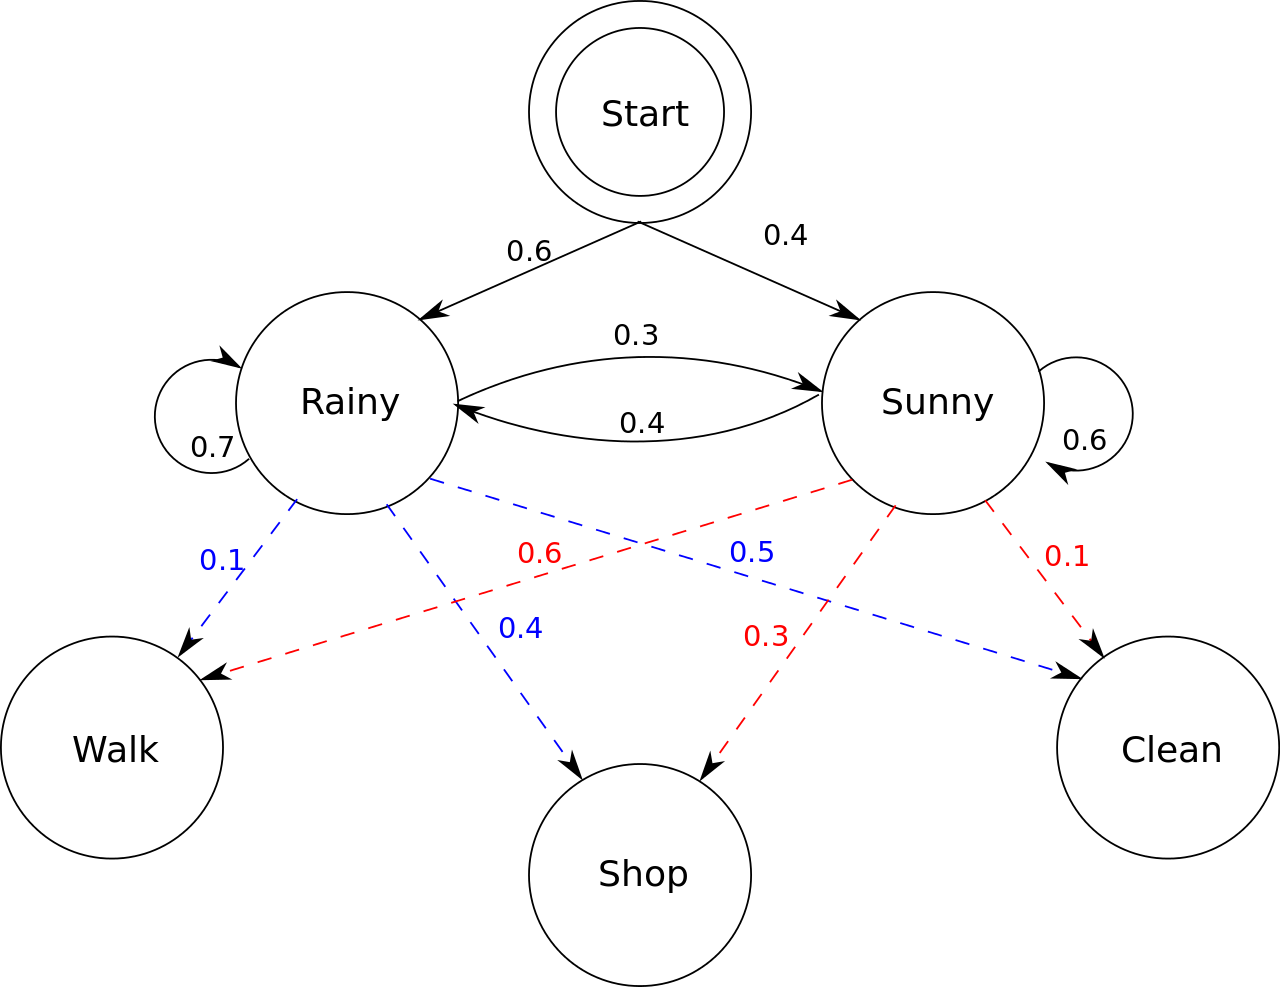
\includegraphics[scale=0.3]{MarkovModel.png}
    %\caption{Example of a Markov Model. It shows the probabilities for the weather to be sunny %or rainy and then, the probabilities for the person to go take a walk, clean or go shopping.}
    %\label{MarkovModel}
%\end{figure}


%-----------------------------------------------------------------------------

\section{Timed Automata}

%-----------------------------------------------------------------------------

%// TODO: Motivation / Why was it created not why I use them

To define a timed automata, we need some more definitions. A timed automata works with timed sequences, timed words and timed languages.\\

\begin{figure}[H]
    \centering
    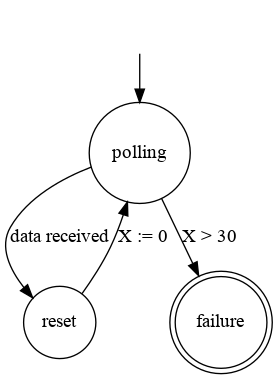
\includegraphics[scale=2.5]{timed_automata.png}
    \caption{Example of a timeout timed automaton. x being one of the clocks that can be used}
    \label{timed_automata_e1}
\end{figure}

For a given input alphabet $\Sigma$, a timed language is defined as a set of timed words over $\Sigma$. A timed word over $\Sigma$ is a pair $(\sigma, \tau)$ where $\sigma$ is a word over $\Sigma$ and $\tau$ is a timed sequence. Lastly, a timed sequence is a sequence of real time values increasing monotonically.~\cite{ALUR1994183} The goal is to map each symbol from the timed word $\sigma$ to a particular time from the timed sequence $\tau$. It allows us to mesure the time between each input symbol.

%// TODO EXAMPLES

\theoremstyle{definition}
\begin{definition}{Timed sequence.}
A timed sequence is an infinite sequence of values increasing monotonically $\tau = \tau_1 \tau_2 ...$ where $\tau \in \R$ and $\forall i : \tau_i > 0$ and $\forall i \in \mathbb{N}: \tau_i < \tau_{i+1}$.
\end{definition}

\theoremstyle{definition}
\begin{definition}{Timed word.}
A timed word over an alphabet $\Sigma$ is a pair $(\sigma, \tau)$ where $\sigma = \sigma_1 \sigma_2 ...$ is an infinite word over $\Sigma$ and $\tau$ is a timed sequence.
\end{definition}

\theoremstyle{definition}
\begin{definition}{Timed language.}
A timed language over an alphabet $\Sigma$ is a set of timed words over $\Sigma$.
\end{definition}

We also need a transition table that can read timed words. We want the transition to consider the input symbol from the input alphabet and the time associated to it when it makes a transition choice. To do so, we associate a set of clocks to our transition table and for each transition, we associate a clock constraint to it and require that the transition may be taken only if the current values of the clocks satisfy this constraint. A clock can be set to zero simultaenously with any transition.

\theoremstyle{definition}
\begin{definition}{Clock constraint.} A clock constraint is defined inductively by
$$\delta := x \le c \mid c \le x \mid \neg \delta \mid \delta_1 \land \delta_2$$ with $x \in X$ and $c \in \Q$. $X$ being a set of cloks.
\end{definition}

\theoremstyle{definition}
\begin{definition}{Clock interpretation.} A clock interpretation $v$ is a mapping $X \to \R$, with $X$ being a set of clocks.
\end{definition}

A clock interpretation $v$ over $X$ satisfies a clock constraint $\delta$ over $X$ iff $\delta$ evaluates to true using the values given by $v$.\\

To use this type of automaton, we need to define a time unit that will be used for the clock interpreation. Each passed time unit, we increase the clock interpreation of every clock by some fixed increment. A simple example is to have a set of clock that are incremented by one every passing second. Here, the time unit is the second and the increment is $1$. Using the same time unit and increment, we can interpert the example given in Figure~\ref{timed_automata_e1} as follows:
\begin{itemize}
\item When data is received, we reset the clock interpretation of the clock $x$
\item If we do not receive data after $30$ seconds, the run is over.
\end{itemize}

The clock constraint here is $x > 30$. This automata can be used to ensure that a data is received at least every 30 seconds.

\theoremstyle{definition}
\begin{definition}{Timed transition table.} A timed transition table $\A$ is a quintuple $(\Sigma, S, s_{0},C, E)$, where:
\begin{itemize}
\item $\Sigma$ is the input alphabet.
\item $S$ is the set of state.
\item $s_{0} \in S$ is the initial state.
\item $C$ is a finite set of clocks
\item $E \subseteq S \times S \times \Sigma \times 2^{C} \times \Phi(C)$ gives the set of transitions where $\Phi(C)$ is the set of clock constraint over $C$. A transition from the state $s$ to $s'$ on input symbol $a$ is represented by a qintuple $(s, s', a, \lambda, \delta)$ where $\lambda$ is the set of clock to be set to zero and $\delta$ is the clock constraint over $C$.
\end{itemize}
\end{definition}

We now have all the needed tools to define properly the type of timed automaton we'll need for this thesis:

\theoremstyle{definition}
\begin{definition}{Timed automaton.} A \gls{ta} $\mathcal{T}$ is a tuple $(\A, W, F)$ where $\A$ is a timed transition table, $W \subseteq S(\A)$ (with $S(\A)$ being the set of state of $\A$) is the set of \textit{success} states and $F \subseteq S(\A) \ W$ is the set of \textit{failure} states. We will only consider deterministic timed automaton in this thesis as ~\cite{10.1007/3-540-63174-7_12} shows that we can transform any \gls{nfa} into a \gls{dfa}.
\end{definition}

\theoremstyle{definition}
\begin{definition}{Run.} We define a run $r$ of a \gls{ta} $\mathcal{T} = (\A, W, F)$, where $\A$ is a transition table $(\Sigma, S, s_{0},C, E)$, over a timed word $(\sigma, \tau)$ as the sequence
$$(\overline{s}, \overline{v}): (s_0, v_0) \xrightarrow[\tau_1]{\sigma_1} (s_1, v_1) \xrightarrow[\tau_2]{\sigma_2} (s_2, v_2) \xrightarrow[\tau_3]{\sigma_3} ...$$
with $s_i \in S$ and $v_i$ is a clock interpretation $C \to \mathbb{N}_0$ $\forall i \ge 0$.
\begin{itemize}
\item $s_o$ is the initial state of $\A$.
\item $\forall x \in C: v_0(x) = 0$
\item $\forall i \ge 1: \exists e \in E$ of the form $(s_{i-1}, s_i, \sigma_i, \lambda_i, \delta_i)$ so that $(v_{i-1} + \tau_i - \tau_{i-1})$ satisfies $\delta_i$ and $v_i$ equals $[\lambda_i \mapsto 0](v_{i-1} + \tau_i - \tau_{i-1})$ with $\tau_0 = 0$.~\cite{ALUR1994183}
\end{itemize}
\end{definition}

%\theoremstyle{definition}
%\begin{example}{Timed automaton.} An example of timed automaton where $C = \{x\}$ is given in figure~\ref{timed_automata_e1}.
%\end{example}
%// TODO more example

Intuitively, a run is the sequence of states and clock interpretations characterizing the \textit{run}/processing of a given timed word to a given timed automata. For each tuple of state and clock interpretation, the clock interpretation is:
\begin{itemize}
\item $0$ for every clock if it is the first of the sequence or
\item the clock interpretation in the sequence $+$ the amount of time unit elapsed with every clock in $\lambda$ being resetted.
\end{itemize}

\theoremstyle{definition}
\begin{definition}{Accepting run.} A run $r$ of a \gls{ta} $\mathcal{T} = (\A, W, F)$, where $\A$ is a transition table $(\Sigma, S, s_{0},C, E)$, over a timed word $(\sigma, \tau)$ is accepting if for $s_{n}$ the last state of $\overline{s}$:
$$s_{n} \in W \bigcup F$$
\end{definition}

\theoremstyle{definition}
\begin{definition}{Rejecting run.} A run $r$ is a rejecting run if it is not an accepting run.
\end{definition}

Using this new definition of run, we can define the language accepted by a \gls{ta} as the set of timed words whose run over \gls{ta} are accepting:

\theoremstyle{definition}
\begin{definition}{Timed language.} Given a \gls{ta} $\mathcal{T} = (\A, W, F)$, where $\A$ is a transition table $(\Sigma, S, s_{0},C, E)$, the language $L \subseteq \Sigma*$ recognized by the \gls{ta} is the set of timed words $w \in \Sigma*$ for which the run of $w$ over the \gls{ta} is accepting.
\end{definition}

We also add the definition of successful and failing runs for future use. Given a \gls{ta} $(\A, W, F)$ and a run $r$, we say it is a successful run if at least one state of the run is a success state and no previous state to this one is a failure state.

\begin{definition}{Success run.} A run $r$ over a \gls{ta} $\mathcal{T}$ is a success run if
$$\exists s_i \in \overline{s} | s_i \in W$$ and $$\forall j < i: s_j \notin F$$.
\end{definition}

\begin{definition}{Failure run.} A run $r$ over a \gls{ta} $\mathcal{T}$ is a failure run if it is not a success run.
\end{definition}

We will use those definition to allows us to use non finite timed words later.


%-----------------------------------------------------------------------------

\section{Applications}

%-----------------------------------------------------------------------------

One of the first question one should ask is how is model checking and formal verification used in the everyday life or at least, for some projects. The following examples of what is currently used in this domain where taken from the most used tools at the time this thesis was written. Unfortunately, this choice is rather subjective as metrics about each possible software usage is not always available but the only thing that interest us is to know how they works and what they have in common.


\subsection{UPPAL}
%-----------------------------------------------------------------------------

\begin{figure}
    \centering
    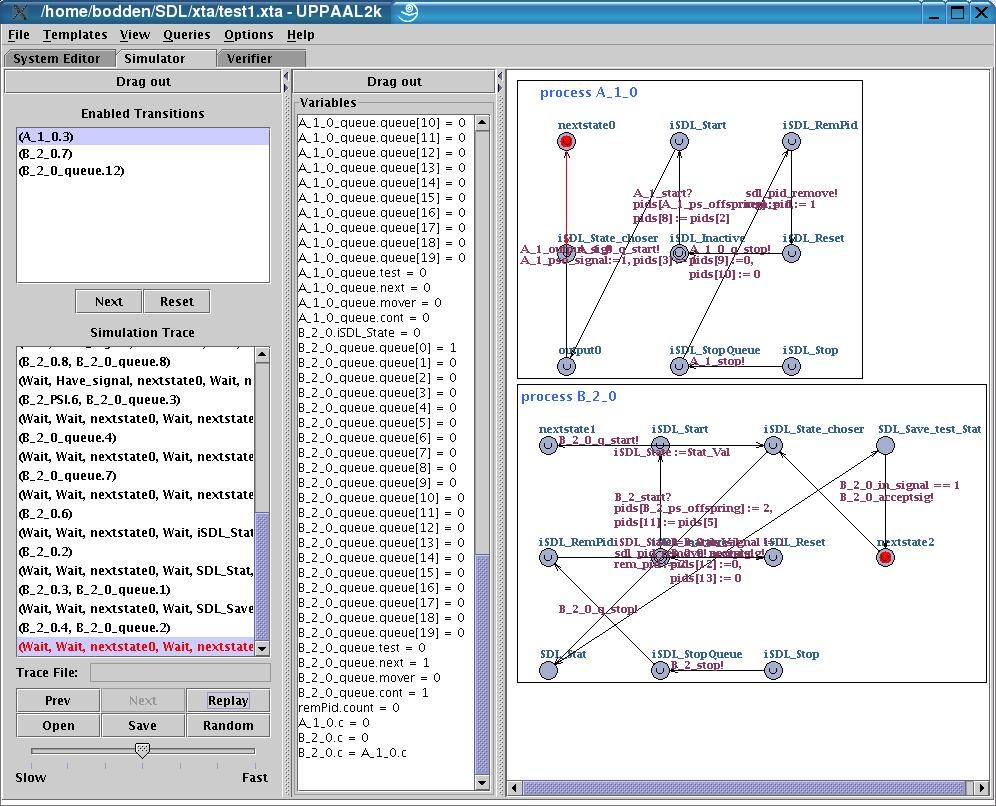
\includegraphics[scale=0.3]{UPPAAL_trace.jpg}
    \caption{Main window of UPPAAL for the simulation part. You can see the execution trace in the lower left corner of the window as well as the model of the system on the right, shown as a TA}
    \label{UPPAAL}
\end{figure}

The first software we came across while searching for such applications was UPPAL. UPPAAL is a rather complete tool to work on model checking and formal verification. With it, one can model a system, simulate and verify it. All the three steps in only one tool~\cite{Bengtsson1996}~\cite{Behrmann2004}~\cite{Larsen1997}.\\

UPPAAL was a great source of inspiration for some features of our own tool. We were specifically interested by the simulation tools which allows to navigate through the execution steps and visualizing what is going on with the model of our system. Also, UPPAAL uses TAs which comforted us in our choice of such tool.\\


\subsection{PRISM}
%-----------------------------------------------------------------------------

// TODO intuition for probabilistic models

\begin{figure}
    \centering
    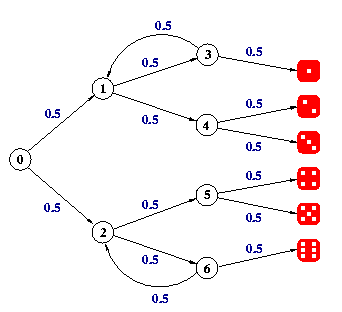
\includegraphics[scale=0.6]{PRISM_model.png}
    \caption{Example of model used by PRISM. This model was generated using the lines of code in figure~\ref{PRISM_code}.}
    \label{PRISM_model}
\end{figure}

We where also interested by PRISM, which is a tool for modeling and verification of probabilistic systems. PRISM supports different kind of probabilistic models like \gls{dtmc}, \gls{mdp}, \gls{pa}, \gls{ctmc} and \gls{pta}.\footnote{Probabilistic Automaton are Markov Chains that also supports deterministic transitions.}~\cite{Kwiatkowska2011}~\cite{Hinton2006}\\

PRISM uses a uniform modeling language for all the probabilistic models that it supports. This is a textual language, based on guarded command notation. See Figure~\ref{PRISM_model}, this model was generated using the following lines of code:

\lstset{
  showspaces=false,
  showstringspaces=false,
  showtabs=false
}

\begin{figure}
\label{PRISM_code}
\begin{lstlisting}[caption="Dice model in PRISM",label={lst:PRISM_code}]
dtmc

module die

// local state
s : [0..7] init 0;
// value of the die
d : [0..6] init 0;

[] s=0 -> 0.5 : (s'=1) + 0.5 : (s'=2);
[] s=1 -> 0.5 : (s'=3) + 0.5 : (s'=4);
[] s=2 -> 0.5 : (s'=5) + 0.5 : (s'=6);
[] s=3 -> 0.5 : (s'=1) + 0.5 : (s'=7) & (d'=1);
[] s=4 -> 0.5 : (s'=7) & (d'=2) + 0.5 : (s'=7) & (d'=3);
[] s=5 -> 0.5 : (s'=7) & (d'=4) + 0.5 : (s'=7) & (d'=5);
[] s=6 -> 0.5 : (s'=2) + 0.5 : (s'=7) & (d'=6);
[] s=7 -> (s'=7);

endmodule
\end{lstlisting}
\end{figure}

Again, this tools uses \gls{fsm} to model different systems.


%-----------------------------------------------------------------------------

\section{Conclusion}

%-----------------------------------------------------------------------------

You should now have a good understanding of \gls{fsm} and some of the various modifications we can add to them. We still have to introduce the background of this work before beginning to mix software development and \gls{fsm} but you should already have a small idea of what possibilities such combination have to offers. We will later explain how we used the \gls{fsm} introduced here as a \gls{dsl} that we uses to describes the testing we want to conduct.


%------------------------------------------------------------------------%
%                                                                        %
%                                                                        %
% CASE STUDY                                                             %
%                                                                        %
%                                                                        %
%------------------------------------------------------------------------%

\clearpage
\part{Case study}

Now that you know what software testing and \gls{fsm} are all about, lets introduce the case that is of interest to us, namely, Nursery! I'll first introduce the Railnova enterprise and the system we will work with all along this thesis. Then I will explain why this work is of critical importance for them and generally speaking, for every software development process.

\clearpage


%-----------------------------------------------------------------------------

\section{Railnova}

%-----------------------------------------------------------------------------

This work is done in partnership with Railnova. Railnova is a technology company that provides telematics and software solutions to the railway industry. Their headquarter is located in Brussels and they count approximatively 30 employees. Some of them coming from the ULB/VUB.\\

The main goal of this work is to develop a better testing suite for their embedded software called \gls{railsteros}. Of course, the developed solution will not be limited to a particular software and our scope is wider than that. Our solution will be considered successful if it meets the following requirements:

\begin{itemize}
\item The system can be used by non-developers
\item It is a time saving technology
\item The solution reduces costs
\end{itemize}


\subsection{Existing system}
%-----------------------------------------------------------------------------

\gls{railsteros} is a software developed at Railnova which purpose is to collect and stream data from a train to a server. This data is then processed to give various insights about the train status. Thus allowing Railnova's client to manage their fleet with ease.\\

The \gls{railsteros} is executed on a dedicated hardware also built by Railnova which is called \gls{rug}. Those \gls{rug} are mainly installed in trains in Germany, France, Belgium, Netherlands and Spain at the time this work was written. More specifically, the \gls{rug} is installed in the engine of trains.\\

This dedicated hardware is used to fetch data from the train's equipments. Those data are then stored in Railnova databases and are used for several applications like maintenance prediction, fuel monitoring, equipments monitoring and so on. We can access informations like remaining fuel (if it is not an electrical engine), the total running time since last power on of the engine, where is the engine located, current speed if the engine is moving and all the data that the client wants to access remotely.\\

Every engine is more or less unique. They can use a wide range of different component and thus have different parameters like their maximal speed when loaded or not, the maximal weight they can carry or even the number of wheels the engine uses. Because of that \gls{railsteros} needs to accept a wide range of different configuration so we don't stream fuel remaining if we are on an electrical engine for example. We can also have two kinds of motors that give information about their speed without using the same type of cable or protocol. To achieve this flexibility, we allow \gls{railsteros} to start only a subset of its internal software using some configuration files. All this software's modules, which we call \gls{daemons}, are small applications used to interface with a given protocol. For example, we have one daemon that is dedicated to GPS location's informations. The set of daemon we use, which is defined in the configuration files, defines what type of engine we can handle and what operations we can do.\\

To retrieve all those informations, we need to use different communication protocols and wires because engines built by different companies will have different behaviors and communication protocols. All of them, we will call interfaces. Each of those interface needs proper test that relies on the used communication protocol with the underlying equipment, we want to be able to describe our needs, explains what data should be fetched by a specific interface, when we should fetch it. As there is a lot of interface, it will take time to implement proper testing for all of them so we will only cover a subset of them in this thesis but we will provide a generic way of implementing test for them all.


\subsection{Railster Universal Gateway}
%-----------------------------------------------------------------------------

As stated before, \gls{railsteros} is running on \gls{rug}. Those hardware are built by Railnova. Actually, the majority of them are in their first version (RUG1) but the RUG2 is on its way. It is important to keep that in mind to understand why we tried to keep this work as generic as possible. Indeed, in a year, maybe less, the majority of the product used will be RUG2 so if the system can only work for a dedicated and specific hardware, we will need to start over all this work for the RUG2.\\

\gls{railsteros} is being developed incrementally since the start of the company. It means that the software becomes harder and harder to maintain with all the new features coming in and the old ones being deprecated or deleted. Actually, there is more than 10 different versions of the software in production and those are not the only existing versions.\\

It is frequent to encounter new bugs after the release of a new version that were supposed to be fixed since earlier versions simply because the new changes re-introduced the problem. This is mainly because Railnova is a young company, a start-up, and the work priority are very end-user scheduled. If a system stops working, a quick fix is developed and pushed to production as fast as possible to avoid loosing too much money but the cost on the long run for this operation can be greater than what we saved by fixing the problem quickly.\\

Say that the problem is fixed by a quick and dirty patch. Then, one year later maybe, a major problem arises because all the fixes deployed are preventing us from adding wanted features. Then, the whole system is to be re-developed from the start. That was what happened when they tried to put \gls{railsteros} on the RUG2. RUG1 was developed the quick and dirty way to be on the market as soon as possible. So a lot of conception errors were made. The software had been modified to a point where it needed all those conception errors from the RUG1 to operate correctly.


\subsection{Short story}
%-----------------------------------------------------------------------------

Some of the \gls{rug} were experiencing troubles during the end of fall 2016. 8\% of the fleet had to be replaced by the team for unknown reasons. After a bit of testing, some members of the team thought that it could come from an unexpected electrical over-consumption of the \gls{rug} while connecting to a GPS antenna. To validate this hypothesis, some testing had to be done. It was the end of summer so the outside temperature was going down so the team thought that maybe it had something to do with that.

The test procedure was defined as follow: First, set the temperature of a thermionic chamber to -10 Celisus to replicate the outside temperature recorded when we experienced the failures. Put a \gls{rug} in it and connect to the serial communication port of the system. Once we are connected, we issue some command to manually choose which GPS protocol to use out of the four of them supported and for each of them, we manually set the emitting power of the GPRS chip in order to reproduce the problem seen on the practical field.\\

Those test were made, approximately 30 for different temperatures of the thermionic chamber, different band and different emitting power. Those took one person an entire day of work! That's because the thermionic chamber needs an hour to set a fixed temperature, the system needs 5 minutes to reboot when we set the band to use and we wait 10 minutes for each test to be sure the problem did not appear (or did). After each test, if we want to do another one, we need to wait for the system to cool down as each time we boot it up, it produces heat.\\

And those tests are just to prove the initial hypothesis. Once this was proved, we wanted to know for sure, what emitting power we could use for each \gls{rug} (not only for one) depending on the band used and the external temperature. This would need hundreds of tests if not a thousand on a lot more than just one \gls{rug} to be able to make enough data and say for sure which levels are safe, which levels are risky and which levels are forbidden to avoid problems in the real world.\\

And that's without mentioning that the thermionic chamber makes a lot of noise to work, wasting an entire room as people can not work long in such a noisy environment.\\

This is where the Nursery project comes in handy. The goal of it is to provide an environment fully automatized to realize all those testing when we want, like during the night so the room stays silent during the day for people to work in, without needing one or more persons to take weeks or years of works.


\subsection{The Railnova Way}
%-----------------------------------------------------------------------------

At Railnova, development in general is lead by the Agile framework. Because of that, software and hardware developed tend to welcome changes and new features are added every week as well as small bug fixes or minor modifications here and there.\\

This tend to make it difficult to keep track of what is working and what is not during the life-cycle of any project. This is where Nursery becomes useful. By providing a tool to check whether or not features are broken after modifications have been applied would be a great time saver. Testing everything manually is a tedious work and waiting for things to break in production environment is a very bad idea like we saw previously.\\

Usually, when one of the \gls{rug} fails in production, the product is called back to the Railnova HQ for \gls{fqm}. \gls{fqm} consists of several phases. During the first one also called "fingerprinting", we try to identify the root cause of the failure. Then, we re-direct the product either to "Debug HW" for hardware debugging if the root cause is hardware linked or to "Debug SW" if the root cause is software linked. After those steps, the problem should be solved. The product is sent to "Fixing" to apply other pending modifications that did not necessitate an immediate return of the product. Finally, the product is sent to "Flash \& Validate" to re-initialize it completely and flag it as "ready to ship".\\


%-----------------------------------------------------------------------------

\section{Conclusion}

%-----------------------------------------------------------------------------

This section should have given you a good idea of why testing is so important at Railnova and in virtually any enterprise. Assuming everything works is just not sufficient and can lead to big trouble with clients.


%------------------------------------------------------------------------%
%                                                                        %
%                                                                        %
% CONTRIBUTION                                                           %
%                                                                        %
%                                                                        %
%------------------------------------------------------------------------%

\clearpage
\part{Contribution}

All the problems described above provides with the necessary information to complete this work. We know what can go wrong, we know what we need and we know that a proper validation of all the developed product is a key for success of any given product on the long run. So having a global view of what software testing is and what is the concrete problem we are dealing with, we will try to design a testing process that can be applied to it and possibly to any other given problem that needs black-box testing. One of our main goal is also to design a tool that will be useful and easy to use but we want it to be powerful enough to be able to handle every test case we might think of.\\


\clearpage


%-----------------------------------------------------------------------------

\section{Requirements analysis}

%-----------------------------------------------------------------------------

First of all, lets take back our software development concepts introduce during the first chapter of this thesis. We have described seven types of testing and now that we know what we are working on, lets try to summarize what type of testing we really need:\\

\begin{itemize}
\item Unit and integration testing: Those kind of testing are great to test the code but that does not give us much informations in terms of requirements. Knowing that all functions work separately is not enough to tell that requirements are met as the program behavior results from the interaction of all those function one with another.
\item System testing: We do want to make sure that our interfaces can run on different hardware. In our case, we want to be able to validate our software for at least RUG1 and RUG2.
\item Functional testing: Testing that the software fullfils the requirements is, of course, our main preocupation. So this type of testing is of main importance.
\item Regression testing: Being able to certify that a new feature or a bugfix does not break the whole system is a key point too. We dont want to re-introduce old bugs or break what is already working well.
\item Acceptance testing: Automatizing client testing is not really in the scope of this thesis. Besides, we assumed earlier that the requirements are good and well validated.
\end{itemize}

Summed up, those are the 3 main requirements we absolutely want in our solution:

\begin{itemize}
\item Functional testing
\item System testing
\item Regression testing
\end{itemize}

We now want to know what we need to satisfy those requirements. We will use them to rate the developed solution in \autoref{chap:Results}. Let us now introduce some concept that will be used to formalize our following ideas:

\theoremstyle{definition}
\begin{definition}{Requirements.} Requirements $R$ is a set of requirements defined by our client(s). Keep in mind that we can be our own client.
\end{definition}

\theoremstyle{definition}\label{def:Testing}
\begin{definition}{Testing.} A test $t$ is used to map a particular requirement $r \in R$ to a satisfaction value:
$$
t: r \to \{True, False\}
$$
When mapped to $True$, we say that the requirement is fullfilled and the requirement is not fullfilled when mapped to $False$.
\end{definition}

This definition is still incomplete, we need to know how the mapping is done and that is the question we are going to answer in this chapter. Also, keep in mind that when we talk about "our software" or "our program", we want to refer to the software being tested. In our case, our software refers to \gls{railsteros} which is the Unix based operating system we want to test.


%-----------------------------------------------------------------------------

\subsection{Functional testing}

%-----------------------------------------------------------------------------

Given a set of requirements, we want to make sure every one of them is fullfilled, using the definition we stated earlier, this is pretty simple to formalize:

\theoremstyle{definition}
\begin{definition}{Functional testing.} Functional testing is used to ensure that the following condition holds:
$$\forall r \in R: t(r) = True$$
\end{definition}


%-----------------------------------------------------------------------------

\subsection{System testing}

%-----------------------------------------------------------------------------

Now, you know what system testing is about. We want to verify if our program can run on more than one system. At Railnova, the practical case we had at hand was about two different hardware, RUG1 and RUG2, both of them handles inputs and outputs differently and we wanted to make sure that our custom Unix based OS would run as expected on both of them.\\

Of course, the newest version, RUG2 had more features than the RUG1 and this lead us to our first observation: Different systems can have the same capabilities but they generaly don't and given that all capabilities should be tested, see functional testing if you don't recall why, the set of tests we should run on a given system is system dependant. Different systems can have all their tests in common if they have the same capbilities, none or some test in common if they don't\\

Again, let's take a practical example: The RUG2 can handle more communication protocols than the RUG1 and can process more information in the same amount of time. So our custom OS should be able to handle those new informations when run on the RUG2 but this is not requiered when run on the RUG1. To fullfil this need, we now know that our solution will have to provide a way of defining the subset of all existing requirement to be tested on a particular system.\\

\theoremstyle{definition}
\begin{definition}{Systems.} $Systems$ is the set of all possible environment on which we want our program to run.
\end{definition}

\theoremstyle{definition}
\begin{definition}{System.} A system $System \in Systems$ a particular environment on which we want our program to behave as expected
\end{definition}

A concrete example of two different systems is a smartphone and a computer. Both are used for different purposes but have some common features (display, user interface, processing power, ...).

\theoremstyle{definition}
\begin{definition}{System requirements.} The subset of requirement that are required for a given $System$ is $R(System)$
\end{definition}

\theoremstyle{definition}
\begin{definition}{Testing.} We can now extend our definition of test by including the system on which the test is done:
$$T: r, system \to \{True, False\}$$
\end{definition}

\theoremstyle{definition}
\begin{definition}{System testing} So now, system testing is simply making sure that, given any $System \in Systems$, the following condition holds:
$$
\forall r \in R(System): t(r, system) = True
$$
\end{definition}

Or simply put, for every requirement of our system, we want to have a test that can evaluate to \textit{true} if the requirement is met and \textit{false} otherwise and we want all those test to evaluate to \textit{true}.


%-----------------------------------------------------------------------------

\subsection{Regression testing}

%-----------------------------------------------------------------------------

In regression testing, we want to make sure that the previous testing are, in the worst case, as efficient as before. If we only managed to fulfill a subset of the needed requirements, we want this subset of requirement still fullfilled in the newest revision of our software.

\theoremstyle{definition}
\begin{definition}{Revision.} We are going to iterate on the tested software to improve it gradually. A revision $V$ of the software $s$ is a mapping of the software to $\real$:
$$
V: s \to \mathbb{N}_0
$$
with the following conditions:
\begin{itemize}
\item $s$ is the latest software revision
\item $s_0$ is the first software revision and $V(s_0) = 0$
\item $\forall x \in \R: V(s_x) > V(s_{x-1})$
\end{itemize}
\end{definition}

Using that, lets extend our test definition to include the software revision:
\theoremstyle{definition}
\begin{definition}{Testing.} Given a requirement $r$, a system $s$ and a software $s_x$:
$$T: r, system,V(s_x) \to \{True, False\}$$
\end{definition}

Having defined those notations, we now have:

\theoremstyle{definition}
\begin{definition}{Regression testing} Verify that, given any $System \in Systems$ and a given software revision $x$, the following condition holds:
$$
\forall r \in R(System): t(r, system, V(s_{x-1})) \rightarrow t(r, system, V(s_x))
$$
\end{definition}

Basically, what worked before must still work now.

\theoremstyle{remark}
\begin{remark} Satisfying the functional testing is sufficent. We don't need to explicitly check the previous version's requirements for divergences as all requirements are mandatory because of functional testing.
\end{remark}


%-----------------------------------------------------------------------------

\section{Requirements satisfaction}

%-----------------------------------------------------------------------------

We now have a good idea of what we want to do, checking various requirements of a given software to make sure they are all satisfied on every different system used. But how to know when a requirement is fullfilled or not? In the chapter dedicated to them, we introduced the notion of failure and accepting states. If we manage to map all the interactions of our system with an input alphabet, we can easilly imagine that a run of a given \gls{fsm} extended with the concept of failure and accepting state can produce the desired mapping for a given requirement. The underlying idea would be to create an \gls{fsm} for every requirement, run them using the defined input alphabet of the software's interactions and check that the resulting mapping is only made of \textit{True} values. If it is the case, we have successfully created a program that satisfies all the given requirements!

All we have to do is to find the best \gls{fsm} type that suits our needs and to formalize the software interactions in a way that allows us to capture and manage them.


%-----------------------------------------------------------------------------

\section{Interfaces}

%-----------------------------------------------------------------------------

%// TODO SCHEMA RUG interfaces Inputes Outputs

%// TODO introduce that in introduction ?
In our practical case, we need to know how the tested program is performing in order to test its requirements. To do that, we need to analyse the output it produces. In this context, outputs can be data, reports, logs, screenshots and many other things as long as they are produced by the analysed program. At Railnova, the \gls{rug} communicate with data servers, it produces particular messages that are saved in Railnova databases. It also can be accessed using a serial communication. Using this serial communication, we can fetch a lot of informations from the \gls{rug} operating system. We want our solution to interface with such data stream. Based on this quick analysis, we can think of separate program whose purpose is to continuously check for new data and fetch them into our solution as \gls{fsm}'s inputs. Let's call those program "Output Providers". So the idea is to setup a set an output providers that will provide informations about how the program is performing. We can imagine a lot of other use cases for those output providers, for example, we can have an output providers that look at a screen whose output is coming from our program and push the screen status into our solution.\\

So, is interfacing outputs from our system enough to build a viable solution? We figure out that it is not. Let's say you want to check that the software produces different outputs based on the room temperature. If you don't have the room temperature, you will not be able to check data's correctness. That's why we also need to fetch inputs of the tested program. Unfortunately, this was not considered early enough in the development process of our solution so the name "Output Provider" was also used for those in the final solution.


%-----------------------------------------------------------------------------

\subsection{Output(/Inputs) providers}\label{sec:providers}

%-----------------------------------------------------------------------------

The goal for those is to fetch or produce data that describes the state of the program or the various variables that can affect its processing/behavior. We decided to allow the user to create any ouptut providers needed. Those provider will then provide data in the form of key-value dictionnary with up to date data in them.
%TODO example here
Each provider being identified, it is then easy in any test to use the data produced by knowing which ouptut provider produces it and which key is used to identify the data. Lets use some more formal definitions for this:

\theoremstyle{definition}
\begin{definition}{Dictionary.} A Dictionary $D$, in this context, is a mapping of key $k \in K$, where $K$ is the set $K(D)$ of all the keys produced by $D$, and discrete values $v \in V$ where $V$ is the set of values $V(D, k)$ that can be assigned to a given key $k$ in this Dictionary:
$$D: k \to v$$
Two dictionary are of the same type if they share the same set of key.
\end{definition}

\theoremstyle{definition}
\begin{definition}{Output/Input providers.} An Output/Input Provider $P$ is a user defined plugin that produces exactly one type of Dictionary $D$. From now on, we will call them \gls{op}.
\end{definition}

So with those definitions, we can have several Output/Input Providers producing the same type of data (Dictionary).
%// TODO better example ,add one example sooner ?
An example for this would be a temperature sensor, one could read the sensor value on a screen or directly on the electrical wire. In this case, we would have one \gls{op} that would fetch the sensor value from the screen and produce a dictionary with only one key $K = { "sensor" }$ and another \gls{op} would do the same but reading the value from the wire.\\

But now, what if we want another sensor, let's say an oil sensor, the set of value that this sensor can be mapped to will probably not be the same and how does one differentiate between one or the other? We could use the \gls{op} as an identification for the Dictionary but instead of that, we decided to add a custom data to all our dictionaries to identify them one from the other:

\theoremstyle{definition}
\begin{definition}{Dictionary (extended).} A Dictionary $D$, in this context, is an identification $i \in \mathbb{N}$ and a mapping of key $k \in K$, where $K$ is the set $K(i)$ of all the keys produced by a given Dictionary identified as $i$, and discrete values $v \in V$ where $V$ is the set of values $V(i, k)$ that can be assigned to a given key $k$ from a given Dictionary identified as $i$:
$$D: k \to v$$
\end{definition}

This now implies that all Dictionary that shares the same identification should produces the same set of keys with the same set of boundaries for their values. A stronger assertion is that each identification of Dictionary denotes a particular context of data. In the previous example, we would now have a new \gls{op} that produces the same set of keys only with a different identification for its Dictionary.


%-----------------------------------------------------------------------------

%\section{Testing environment}

%-----------------------------------------------------------------------------

% The testing environment should emulate perfectly any given train/engine. Each train have a set of interfaces that are plugged into the tested system. What we mean by "interface" is one particular input type, those will be described later on. The system that will emulate the train (or the testing environment) will be given a set of "scenario"\\

% Those scenario will describe what can happen to the system and how it will react to it. A strong constraint in the case that concerns us is that, those scenario will be written by people with poor or no knowledge of advanced programming so we need to provide a simple yet powerful language to write those stories.\\

% We will assume that our testing environment have a way of sending every kind of inputs to the software being tested and retrieved every kind of outputs from it. Of course, in some case this is very difficult to achieve. Lets consider a practical example that is happening for the \gls{rug} case.\\

% The \gls{railsteros} communicates with a GPS/GSM chipset that is connected to antenna that are not under our control. This is an issue because under those circumstances, if the antenna can behave differently in production than during our tests sessions so some faults can goes undiscovered until that.\\

% Some solutions exists for this kind of problems like having our own antenna or using development boards for this chipset. We could also try to write some kind of simulator that will interface with the GPS/GSM chipset but we would need to reverse engineer the whole GSM/GPS networks or at least one particular antenna which would be really time and resources consuming. Not to mention that it will also probably be way more expensive than fixing hypothetical faults when they arise in the production environment. So the complex interfaces needed for those kind of technical component and specifically, their implementations are not a simple matter and are way beyond the scope of this thesis so we will not talk more about them. \\

% In this thesis and for case like this one, we will simply consider that it is not a part of the system that we can test. So every component that are part of the whole system being tested are provided with some interface that allows us to communicate with them, sends and retrieves data.\\

% With that in mind, we want to be able to describe what happens on the input side of the studied system and then, what are the expected results or outputs produced. For example, when you put some money in a vending machine to buy a soda, the system is the vending machine, you don't know how it works (or at least, most people don't), you feed it some inputs (some money) and you expect a given output (a soda) (figure~\ref{vm-io}). This is exactly what you want to describe in your tests.\\

% \begin{figure}
%     \centering
%     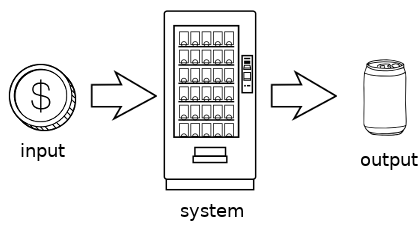
\includegraphics[scale=0.8]{vending-io.png}
%     \caption{The vending machine I/O mapping}
%     \label{vm-io}
% \end{figure}

% A naive idea to do so could be to write a file mapping every possible inputs to every possible outputs and claim that our process works only when no unpredicted input/output pair occurs during some run of it (figure~\ref{io_map1}). But then, what if we want to produce a different output depending on how many times we seen some given output? With this first idea, it would not be possible to handle this as we don't keep track the current state of the process. We don't have a way of counting how many given inputs have been encountered since the start of the process.\\

% \begin{figure}
%     \centering
%     \begin{tikzpicture}[ele/.style={fill=black,circle,minimum width=.8pt,inner sep=1pt},every fit/.style={ellipse,draw,inner sep=-2pt}]
%     \node[ele,label=left:$a$] (a1) at (0,5) {};
%     \node[ele,label=left:$b$] (a2) at (0,4) {};
%     \node[ele,label=left:$c$] (a3) at (0,3) {};
%     \node[ele,label=left:$d$] (a4) at (0,2) {};
%     \node[ele,label=left:$e$] (a5) at (0,1) {};

%     \node[ele,,label=right:$1$] (b1) at (4,5) {};
%     \node[ele,,label=right:$2$] (b2) at (4,4) {};
%     \node[ele,,label=right:$3$] (b3) at (4,3) {};
%     \node[ele,,label=right:$4$] (b4) at (4,2) {};
%     \node[ele,,label=right:$5$] (b5) at (4,1) {};

%     \node[draw,fit= (a1) (a2) (a3) (a4) (a5), minimum width=2cm, label=above:$Inputs$] {} ;
%     \node[draw,fit= (b1) (b2) (b3) (b4) (b5), minimum width=2cm, label=above:$Outputs$] {} ;
%     \draw[->,thick,shorten <=2pt,shorten >=2pt] (a1) -- (b4);
%     \draw[->,thick,shorten <=2pt,shorten >=2pt] (a1) -- (b2);
%     \draw[->,thick,shorten <=2pt,shorten >=2] (a2) -- (b2);
%     \draw[->,thick,shorten <=2pt,shorten >=2] (a3) -- (b1);
%     \draw[->,thick,shorten <=2pt,shorten >=2] (a4) -- (b3);
%     \end{tikzpicture}

%     \caption{Not explicit schematisation of a valid mapping of inputs to outputs, all possible cases are not taken into account. On the left, the input we send into the system and on the right, the outputs we can receive. Arrows shows what are the expected outputs for a particular input}
%     \label{io_map1}
% \end{figure}

% This first idea gave us an important lesson, we need to keep track of the state of the process or at least of what happened before the current time. This does correspond to what we call \gls{fsm} and this is why we introduced them earlier.


%-----------------------------------------------------------------------------

\section{Framework}

%-----------------------------------------------------------------------------

We still need a way for the user to describe how the testing will be done. We decided to describes that using an \gls{fsm} for each requirement testing and to call such \gls{fsm} a scenario, we will refine this definition later after having explained which \gls{fsm} we will use:

\theoremstyle{definition}
\begin{definition}{Scenario.} A scenario is an \gls{fsm} whose goal is to perform a test.
\end{definition}

In theoretical \gls{fsm}, the number of states is bounded above by the system's internal memory. If we want to test every possible state by explicitely stating what should happen in every memory configuration, it would gives us $2^x$ states to analyze (where $x$ is the system's internal memory expressed in bit). Let's say that this memory can be around two to eight gigabits and this is raising every year. So we would have to describe what should happen in $2^{8*10^9}$ different states. We don't say that this is not possible but if we can do the same using a model of how the system should behave (a scenario) with less than 25 states for example, it should be easier for any human being.\\

So to address this problem, we need to abstract the state definition. We'll aggregate formal states into a more complex structure that we will still call a state but for the user, it will just be something like "initialization state", "error state", "processing data state" and so on. A state will simply be a set of computation that needs to be applied.
We want to be able to react when leaving or entering a state, we are now programming so we will probably need to free ressources or allocate them for example. It would also be nice to be able to repeat some operation when we receive some input symbol. Of course, this behavior could be achieved using more states and transition but lets try to keep it simple, fewer states and transitions means less complexity, code and more readability. So we introduce three optional functions, one for the computation needed when we reach the state, one for when we leave the state and the last one for the computation we need to do every time a new symbol is read.\\

Speaking of input symbols, we talked about data providers in section \ref{sec:providers}. We want to use them to get input symbols. So let's define our input alphabet as a set of dictionary:

\theoremstyle{definition}
\begin{definition}{Input alphabet.} The input alphabet we will be working with is a set $\Sigma$ of dictionaries $D$.
\end{definition}

To choose the type of \gls{fsm} that best suits our needs, we need some kind of ranking system based on what we learn in the chapter \textit{Formal Verification and Model Checking}~\ref{ModelChecking}. We decided to use the following criteria:
\begin{itemize}
\item We want to make sure that a particular \gls{fsm} type is possible to apply in our case. If it is an abstract \gls{fsm} that uses infinite memory or another paradigms that is impossible to implement on modern computer, we know that we can discard it.
\item How easy it is to describe a system's behavior with such \gls{fsm}? If it takes to much times or if we find it too difficult for non-technical people to describe a system's behavior using that particular \gls{fsm} type, we know that it will probably be deprecated over time and wont be used as it should be.
\item If the chosen \gls{fsm} introduces restriction on what can be described, those restriction must not prevent us from doing every testing needed. And if it introduces new possibilities that allows us to describe more system's behaviors, the complexity that it introduces into the system should be worth it.
\end{itemize}
%// TODO ^ this earlier
%// TODO describe what we want to describe

We can summarize with the following questions:

\begin{itemize}
\item Is it possible to implement?
\item Is it user friendly?
\item Does this introduces restrictions?
\end{itemize}

Now to the choice of \gls{fsm} model, why don't we simply pick the most simple case of \gls{fsm}? The reasons are very simple, take this case: You want to be able to detect a failure that happen if you receive a given data more than 10 seconds after some given data. How can you do this? Or even simpler, you want to detect a failure if you didn't receive any data for 30 seconds.\\

With a basic \gls{fsm} that do not consider time, we would have to add a new input symbol to be used when no input data is received and assume that you use a reference time unit and that each time unit passed, you should receive a data or the newly introduced input symbol when no data is received. We need to add states for each seconds passed, so if we want to wait 30 seconds, we need 30 states with 30 transitions for each seconds and 30 transitions for the event of "a data has been received" that will go back to initial state. And all of this needs to be written by someone. You can easily see why this is impracticable. So clearly, in this case, \gls{fsm} are too limited if we want to handle this in a simple and practicable way, that is, by limiting the number of states the user will need to use. And of coruse, this is no longer a basic \gls{fsm} so clearly, those are not enough for us.\\

%// TODO why is it complex ? why is it lot of work ?
Now with the \gls{afa}, the complexity of implementation required by this paradigm is important, we need to run multiple automaton, construct execution trees and analyze them. Compared to a simple \gls{fsm} implementation, this is a lot of work. So is it worth it? To answer this question, we need to find practical cases where such a paradigm would become indispensable and such case should be really difficult to implement into a classic \gls{fsm} to justify choosing \gls{afa} as our main choice for the implementation of Nursery. Based on the concrete needs we had when we analyzed this possibility, we choose not to consider it as a good solution because none of the cases we had prepared (see section~\ref{section:ourcase}) needed such complexity and using this would have made it difficult to design test by inexperienced users. This also follows from the fact that we wanted to avoid dealing with concurrency.\\

There is a wide variety of \gls{fsm}, there isn't any limit on how many \gls{fsm} type you can think of but when we started implementing our solution, the best \gls{fsm} that our 3 ranking questions left us with was timed automaton. Those \gls{fsm} are really well adapted for our use case. Being able to manipulate time directly in our transitions and state gives us a lot of ease to write the code and its also very powerful too! With it, we are able, for example, to send data with a variable interval between them and then receive data accordingly. You can also decide to create a clock for timeout that will be reseted each time you receive a given data. There are really a lot of use case and some more will be described later on.\\

This choice of tool is also motivated by the fact that writing and understanding automaton is a very easy process. Designing a \gls{ui} to create automata and generating valid scenario out of it is a relatively easy process so this could be a way to meet the strong requirement that our solution shall be easy to use for not seasoned programmers.\\

Let's now refine a bit our definitions of a scenario:
\theoremstyle{definition}
\begin{definition}{Scenario.} A scenario is a timed automaton whose goal is to perform a test.
\end{definition}

We also want to improve the input alphabet we will be working on, if we include the clocks in it, we will be able to perform operation every given time interval:
\theoremstyle{definition}
\begin{definition}{Input alphabet.} The input alphabet we will be working with is a set $\Sigma$ of dictionary $D$ and a set of clocks $C$.
\end{definition}

At each time step, we will receive a set of dictionary for every input received at this time and the set of clock of the \gls{ta} updated with the current time step.


%-----------------------------------------------------------------------------

\section{Conclusion}

%-----------------------------------------------------------------------------

We introduced the concept of portability when we talked about system testing and versioning when we talked about regression testing and with the third testing, functional testing, we stated that we want the software to run accordingly to our requirement on any system and for every revision of it and we also explained why we wanted to use time automaton. All of those aspect and tools will be used in the following chapter to explain how the final system works.

%// TODO explain I/O producers example and usage is coming
%// TODO exaplain whe are going to explain how to write scenario / TA
%// TODO find ways to shows failing / succeeding relate to passing test


%------------------------------------------------------------------------%
%                                                                        %
%                                                                        %
% RESULTS                                                                %
%                                                                        %
%                                                                        %
%------------------------------------------------------------------------%

\clearpage
\part{Results}
\label{chap:Results}

This part is a in depth description of how the implemented system works, how it has been developed and what it can and cannot do. This is a more technical part dedicated to the implementation where we will not talk a lot about the mathematical concept behind it as those have already been explained before.\\

\clearpage



%-----------------------------------------------------------------------------

\section{Domain-specific language}

%-----------------------------------------------------------------------------

We start by explaining how we created the \gls{dsl} used to describes our scenario in Python. All the code produced will be Python code but we took the liberty to talk about \gls{dsl} to describes the functions and methods presented in this section even if it is still Python which is a \gls{gpl}. We want to allow the user to do the following operations:

\begin{itemize}
\item Create a scenario
\item Add states to scenario
\item Add transition to states
\item Set success and failure states
\item Set initial state
\item Set enter/leave processing for every states
\item Set update processing for every states
\end{itemize}

As we use Timed automata, we also need to uses clocks:

\begin{itemize}
\item Add/Remove/Set/Reset clocks
\item Get given clocks time
\item Trigger transition using clocks
\end{itemize}

Regarding the data sources, we want our transitions to be able to react on such data and to explicitly specify which kind of data our scenario will be working with. We should now distinguish between two kind of data, either the data is a discrete value, like e-mails, you want to be notified when you receive one or the data is continuous like the room temperature. We want to be able to get both of those data types:

\begin{itemize}
\item Set data sources to be used
\item Receive discrete data as they appear from data source
\item Ask for continuous data reading from data source
\end{itemize}


\subsection{Create a scenario}
%-----------------------------------------------------------------------------

Creating a scenario is done by creating a subclass of \textbf{AbstractScenario} like so:

\begin{figure}[H]
    \begin{lstlisting}[caption="Creating a scenario",label={lst:python-create-scenario}]
from .AbstractScenario import AbstractScenario

class Scenario(AbstractScenario):
    def __init__(self, settings={}):
        AbstractScenario.__init__(self, settings=settings)
    \end{lstlisting}
\end{figure}


\subsection{Add states to scenario}
%-----------------------------------------------------------------------------

When adding a state to a scenario, you can also gives it several function that will be used for update, enter and leave trigger. You can also specify if it is a failure/success state. We satisfy the following requirement with one line of code:
\begin{itemize}
\item Add states to scenario
\item Set success and failure states
\item Set enter/leave processing for every states
\item Set update processing for every states
\end{itemize}

%// TODO explain leave, update, enter handlers. Function ect ect

\begin{figure}[H]
    \begin{lstlisting}[caption="Add states",label={lst:python-add-state}]
state = self.add_state("name", enter=self.on_enter, update=self.on_update, leave=self.on_leave, status=state_status)
    \end{lstlisting}
\end{figure}


\begin{figure}[H]
    \begin{lstlisting}[caption="Various usage of self.add\_state",label={lst:python-add-state-examples}]
from .AbstractScenario import AbstractScenario

NORMAL = 0
SUCCESS = 1
FAILURE = -1

class Scenario(AbstractScenario):
    def __init__(self, settings={}):
        AbstractScenario.__init__(self, settings=settings)

        init = self.add_state("init", enter=self.on_enter, update=None, leave=None, status=NORMAL)
        failure = self.add_state("failure", enter=None, update=None, leave=None, status=FAILURE)

        # Equivalent without handler
        success = self.add_state("success", status=SUCCESS)

        # Normal state with no handler
        foo = self.add_state("foo")

        # Only one update handler
        bar = self.add_state("bar", update=self.on_update)

    def on_enter(self):
        # Do some stuff
        pass

    def on_update(self, t, d):
        # Do some stuff
        pass
    \end{lstlisting}
\end{figure}

In the listing~\ref{lst:python-add-state}, \textbf{state\_status} is $0$ by default, a value of $-1$ indicates a failure state and a value of $1$ indicates a success state. Code starting with \textit{self.on\_} are function defined elsewhere, you can use whatever name you want to name them. The function definition of any update handler should take $t$ and $d$ as inputs: $t$ being the clock of the current state. This clock is reset when we enter the state and $d$ is a possibly empty array of dictionnaries given by the data sources used (we will define that later).



\subsection{Add transition to state}
%-----------------------------------------------------------------------------

To do so, use the function \textbf{add\_transition} from any starting state and give it the goal state to which we should transition in case of success and a transition handler. The handler should return True if the transition must be taken and False otherwise. It takes $t$, the state clock as an input (see section~\ref{ManipulateClocks} for the state clock) and $d$ a list of dictionnaries given by the data sources used (again, this will be defined later).

\begin{figure}[H]
    \begin{lstlisting}[caption="Add transition to any state",label={lst:python-add-transition}]
# Example using a python labmbda function
from_state.add_transition(goal_state, lambda t, d: t > 60)

# Example using a function defined elsewhere
from_state.add_transition(failure_state, self.transition_handler)
    \end{lstlisting}
\end{figure}


\subsection{Set initial state}
%-----------------------------------------------------------------------------

Using a states previously created, a simple call to \textbf{self.tsm.set\_initial\_state} allows us to set the initial state.

\begin{figure}[H]
    \begin{lstlisting}[caption="Set the initial state",label={lst:python-set-initial-state}]
self.tsm.set_initial_state(state)
    \end{lstlisting}
\end{figure}


\subsection{Manipulate clocks}\label{ManipulateClocks}
%-----------------------------------------------------------------------------

We have a global clock used for every state. This clock is resetted every time we enter a new state. We can also create new clocks when needed using the functions in listing~\ref{lst:python-clocks}. The main clock is used as the $t$ parameter for update handlers and transition functions. This satisfies the following points:
\begin{itemize}
\item Add/Remove/Set/Reset clocks
\item Get given clocks time
\item Trigger transition using clocks
\end{itemize}


\begin{figure}[H]
    \begin{lstlisting}[caption="Set the initial state",label={lst:python-clocks}]
# Main clock. This clock value is the t parameter of update handlers and transitions
self.clock.get_elapsed()

clock1 = Clock()
clock1.start()
sleep(1)
clock1.get_elapsed() # should give 1
clock1.reset()
clock1.get_elapsed() # should give 0
clock1.stop()
    \end{lstlisting}
\end{figure}

This feature allows us to create clocks that are not dependant of any state. You could see the states clock as a clock that is resetted at every transition. More formally, this clock is always in the set of resetted clocks for the transition function: Given a \gls{ta} $\mathcal{T} = (\A, W, F)$ where $\A = (\Sigma, S, s_{0},C, E)$, we call the state clock $m$ with $m \in C$. This clock will be used as the state clock and $\forall t \in \A: m \in t(\lambda)$ where $t(\lambda)$ is the $\lambda$ set of clocks to be resetted with this transition.\\

The additional clock we can create are not related to any specific state by default. They work like any clock as defined in \gls{ta} definition.


\subsection{Manipulate data sources}
%-----------------------------------------------------------------------------

Here we want to satisfy the last three requirements:
\begin{itemize}
\item Set data sources to be used
\item Receive discrete data as they appears from data source
\item Ask for continuous data reading from data source
\end{itemize}

First, any scenario needs to states which data sources will be used. For a continuous data source, we will receive a data dictionary from a given data sources for every call of \textbf{self.ask\_data("DATA\_SOURCE")} where \textbf{DATA\_SOURCE} is the name of the data source. For discrete data, the $d$ parameter for update handler and transition will be a dictionnary every time new data is available without further function calls.

\begin{figure}[H]
    \begin{lstlisting}[caption="Set data source",label={lst:python-data-sources}]
# Set data sources
self.l_data_type.append("EMAIL")
self.l_data_type.append("ROOM_TEMP")

# Asking data
self.ask_data("ROOM_TEMP")

# Checking data
if d is not None and d['type'] == "ROOM_TEMP":
    # Process
    pass
    \end{lstlisting}
\end{figure}


\subsection{Determinism}
%-----------------------------------------------------------------------------

A question you should be asking yourself now is, is this system deterministic? The answer is not yet. In the current state, if we have two transition that are satisfied from the same state at the same time, we do not know which one should be taken. To solve this problem, we mapped every transition to a integer in $\mathbb{N}_0$ always growing for each added transition. Transition are then evaluated from the lowest integer value to the biggest. The first succeeding transition will then be taken and we completely ignore the following ones. When designing scenarios, one should keep that in mind otherwise some unexpected cases can appear. Every time the scenario is used, this mapping should stay the same. It can only be modified by modifying the source code itself. This is why every scenario should be versionned too. At Railnova, we uses Github for that purpose. It is not garanteed that two different versions of a scenario will have the same behavior but for a given version number, every time the scenario is used, it will have the same behavior.


%-----------------------------------------------------------------------------

\section{Nursery}

%-----------------------------------------------------------------------------

As we already mentionned earlier, we uses Python as the programming language. Most internal tools used at Railnova are written in Python because it is fast and easy to prototype ideas with it. Most of the employees there have at least basic knowledge of it which is not necesseraly the case with other language such as C or C++. We wanted the system to be used by everyone with limited computer science knowledge so we decided to used Python too.


\subsection{Architecture}
%-----------------------------------------------------------------------------

Nursery works on top of two main features, logging and reporting. Logging allows us to keep track of Nursery outputs. For every test, a file is created to log every one of them. Each line of output has an additional property which is the level of urgency of the output. The possible levels are the following:

\begin{itemize}
\item DEBUG. Used to output values that are not vital to understand what is going on but are of absolute necessity for debugging purposes.
\item INFO. The default output level. Simple information messages.
\item WARNING. Used for warnings. When an expected error occurs which is not breaking the system.
\item ERROR. Error messages. For the messages that should not happen.
\item CRITICAL. When the system is broken, this kind of message should be used.
\end{itemize}

The goal of this logging feature is to produce files that contains every single information needed to identify the reasons of test failure and contains all the tests parameters. A lot of time was put into this feature to allow for useful context related informations for every line of output which, we find, is a key component for Nursery.\\

On top of this logging facility, we added a reporting feature. This one is intended to update bug trackers, product tracking facilities or anything else needing informations about the status of a particular hardware or software. Typically, this is used to update a product tracking server, Redmine, used at Railnova to keep an history of what happened in fingerprinting. When a test is done, the results is added on Redmine by saying: "Test <name> success/failure on RUG <serial number>", of course, other informations are added such as the test version, test criteria and why the test failed. This can also be used to keep track of the status of a production line. At every stage of the production line, we can update the status of the product being build with this reporting tool.\\

Each type of reporting is described by a Python file. Adding one is a very easy process that any developer can achieve. To match the correct reporting to the test being performed, we specify a product type. Those are pre-defined in a configuration file that will be described later on. Each product type maps to a particular reporting type. For example, if we say that we want to perform a test on a product of type "RailsterOS", on the software then, we can have a reporting that will send reports by mails or send them on a bug tracker.\\

\begin{figure}
    \centering
    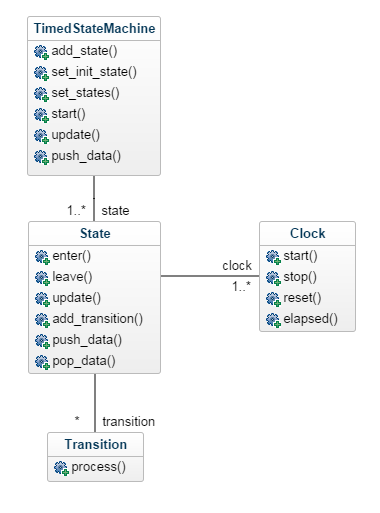
\includegraphics[scale=0.8]{class_diagram.png}
    \caption{Class diagram of the timed automata implementation. Each scenario is a timed automata and each test is composed of one or many scenario.}
    \label{class_diagram}
\end{figure}

\begin{figure}
    \centering
    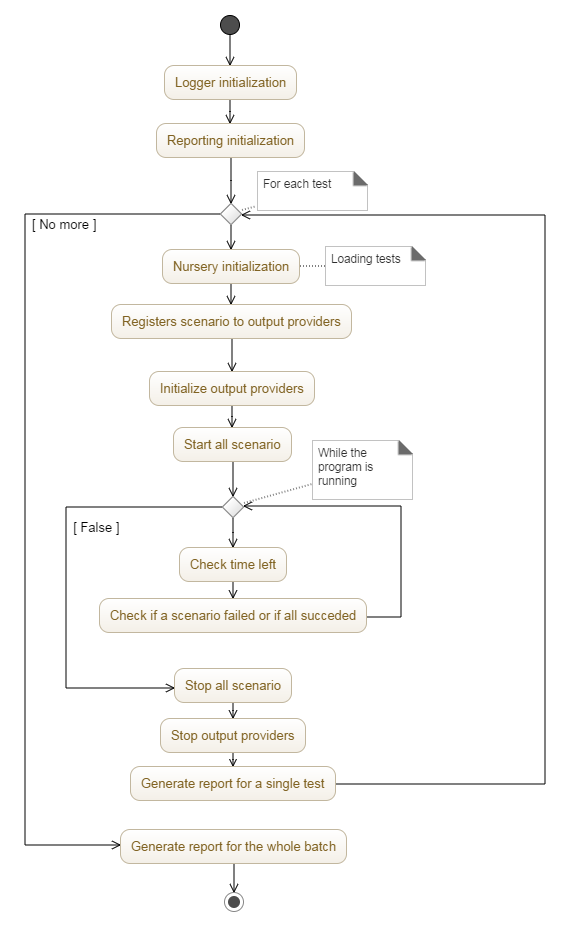
\includegraphics[scale=0.5]{activity_diagram.png}
    \caption{Activity diagram of the whole test processing. A batch of test is simply a list of one or more tests.}
    \label{activity_diagram}
\end{figure}


\subsection{Configuration}
%-----------------------------------------------------------------------------

The whole systems is based on one configuration file. This file contains all available test for Nursery. It also contains all output providers, all batch of tests and the list of all product that can be tested matched with their corresponding reporting. An output provider is a script that everyone can write used to provide data to the test. We used it, for example, to gather data in an online database. Those data are then send to each test as we receive them. A batch of test is just a list of test that needs to be performed in the given order.\\

Like we say earlier, we also have a concept of product type. Each possible product type is mapped to a given reporting file using a code similar to the one shown in the listing~\ref{lst:l_product_type}. The list of "tests batches" are listed using the code of listing~\ref{lst:l_batch} and finally, each test is defined using a code similar to the listing~\ref{lst:l_test_op}.\\

Several parameters are needed to add a test. \textbf{name} and \textbf{description} are simply used to display documentation about them. \textbf{l\_product} is a list of product to which the test applied. This is purely used to warn the user if he tries to perform a test meant for RailsterOS on a battery pack for example. The duration specify the maximum duration of the test in second. After that, the test fails automatically. Finally, the \textbf{l\_scenario} parameter is the most important one. It specifies all the \gls{fsm} that are run in parallel to obtain the desired behavior. Most of the test used only one \gls{fsm} because it proved difficult to conceive test thinking about multiple \gls{fsm} at once. A typical case where it is useful to run multiple \gls{fsm} at once is for timeout check. One of them checks continuously for timeout between data gathered by the output provider and the other one performs the test without having to manage this problem.\\

\begin{figure}
    \label{masterlist_op}
    \begin{lstlisting}[caption="Output provider configuration",label={lst:masterlist_op}]
masterlist_op = [
    { "type": "WANESY", "name": "WanesyProvider" },
    { "type": "SERIAL_WANESY", "name": "SerialWanesyProvider" },
]
    \end{lstlisting}
\end{figure}

\begin{figure}
    \label{l_test_op}
    \begin{lstlisting}[caption="Tests configuration",label={lst:l_test_op}]
l_test = [
    # Efficiency Vs Current
    {   "name": "efficiency_vs_current",
        "l_product": ["battpack"],
        "description": "Test the efficiency against the current",
        "duration": 24*3600,
        "l_scenario": [
            {"name": "EfficiencyVersusCurrent", "settings": {}},
        ], },

    # CAT test
    {   "name": "cat",
        "description": "CAT simulator",
        "duration": 500,
        "l_scenario": [
            {"name": "ReplaySimulator", "settings": {
                "filename": "cat.simulator",
                "csv_delimiter": ",",
                "muted": True,
            }},
            {"name": "CATCheck", "settings": {}},
            {"name": "TimeoutCheck", "settings": {}},
        ], },

    # Charge Battery Pack
    {   "name": "chargebattpack",
        "description": "Charge fully the battery pack",
        "duration": 7200,
        "l_scenario": [
            {"name": "ChargeBattPack", "settings": {}},
        ], },
]
    \end{lstlisting}
\end{figure}

\begin{figure}
    \label{l_batch}
    \begin{lstlisting}[caption="Batch of tests configuration",label={lst:l_batch}]
l_batch = [
    {
        "name": "fingerprint",
        "l_test": [
            "serial",
            "symshow",
            "twctrl",
            "ifconfig",
            "qstat",
            "1970check",
            "gps",
            #"timeout",
        ]
    },
]
    \end{lstlisting}
\end{figure}

\begin{figure}
    \label{l_product_type}
    \begin{lstlisting}[caption="Products configuration",label={lst:l_product_type}]
l_product_type = [
    {
        "type": "none",
        "description": """
            Applied to all hardware/software. Mainly used to disable reporting
        """,
        "reporting": "NoneReporting",
    },
    {
        "type": "rug1",
        "description": """
            Railster Universal Gateway 1
        """,
        "reporting": "RugReporting",
    },
    {
        "type": "ros",
        "description": """
            Railster-OS. Used for software testing
        """,
        "reporting": "NoneReporting",
    },
    {
        "type": "battpack",
        "description": """
            Testing for the battery pack
        """,
        "reporting": "NoneReporting",
    },
]
    \end{lstlisting}
\end{figure}


\subsection{Command line tools}
%-----------------------------------------------------------------------------

To run Nursery, the user can use a command line tool taking several inputs. Those inputs are the following:

\begin{itemize}
\item product: Type of hardware tested
\item serial: RUG serial number to fetch informations with output providers. Needed only for \gls{rug} testing.
\item password: Password, if any, for serial connection.
\item log: Level of informations displayed in the log files, can be "critical", "warning", "info", "error" or "debug"
\item quiet: Used to remove console outputs
\item batch: Batch name to be performed. This override the \textbf{test} parameter
\item test: Name of the test to be performed
\item logpath: Specify where to put the resulting log file
\item checkmaster: used to verify the configuration file. Checking if no errors where introduced
\item report: Indicate whether or not we want to generate a report. This allows us to disable the reporting feature
\item fqm: Shortcut to run a batch named "fingerprint" and generating reports for those tests
\end{itemize}


\subsection{Web-administration}
%-----------------------------------------------------------------------------

\begin{figure}
    \centering
    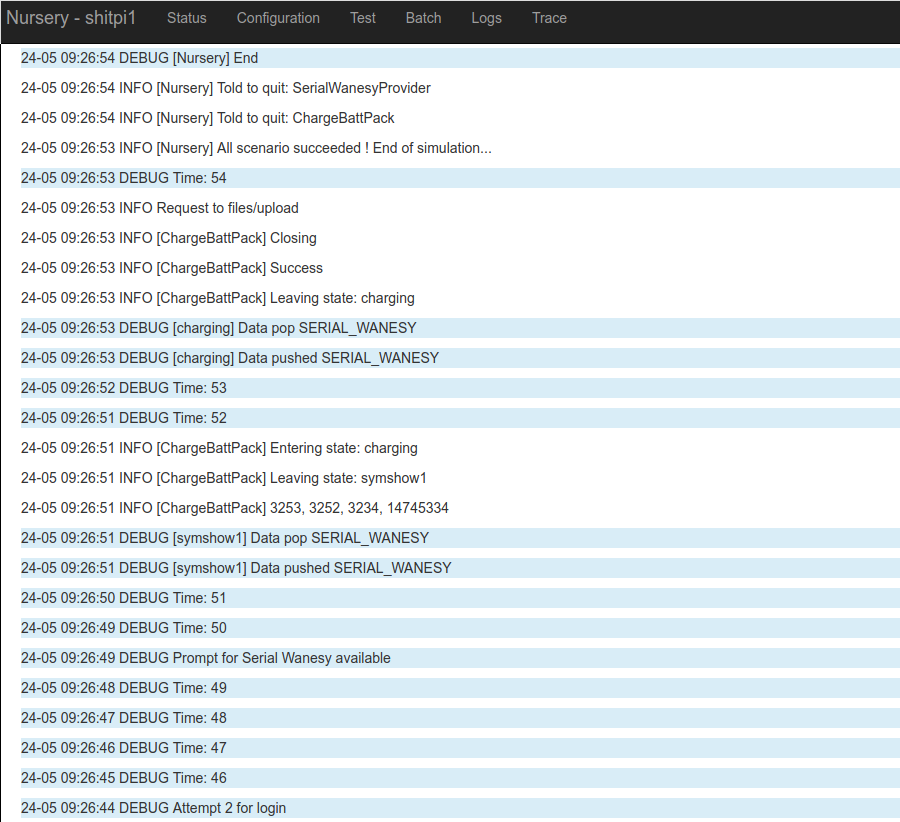
\includegraphics[scale=0.4]{wa_status.png}
    \caption{Main interface for the web-admin tool. Here we can see the last log file generated.}
    \label{wa_status}
\end{figure}

A web-administration tool was also developed. Allowing users to manage testing easily. All features covered by the command-line tool are available through the web-administration tool. We also added three others feature, the first one is the ability to browse all available tests and their documentation (figure~\ref{wa_tests_doc}) and the second one is the ability to see how a test was processed by displaying a automatically generated graph of the test and highlighting nodes of the graph depending on the current step selected in the trace file displayed next to the graph (figure~\ref{wa_trace}). Finally, the ability to manage log files is a feature that is not covered by the command line tool (figure~\ref{wa_logs}). All those features makes the web-administration tool a lot easier to use than the command line tool.\\

\begin{figure}
    \centering
    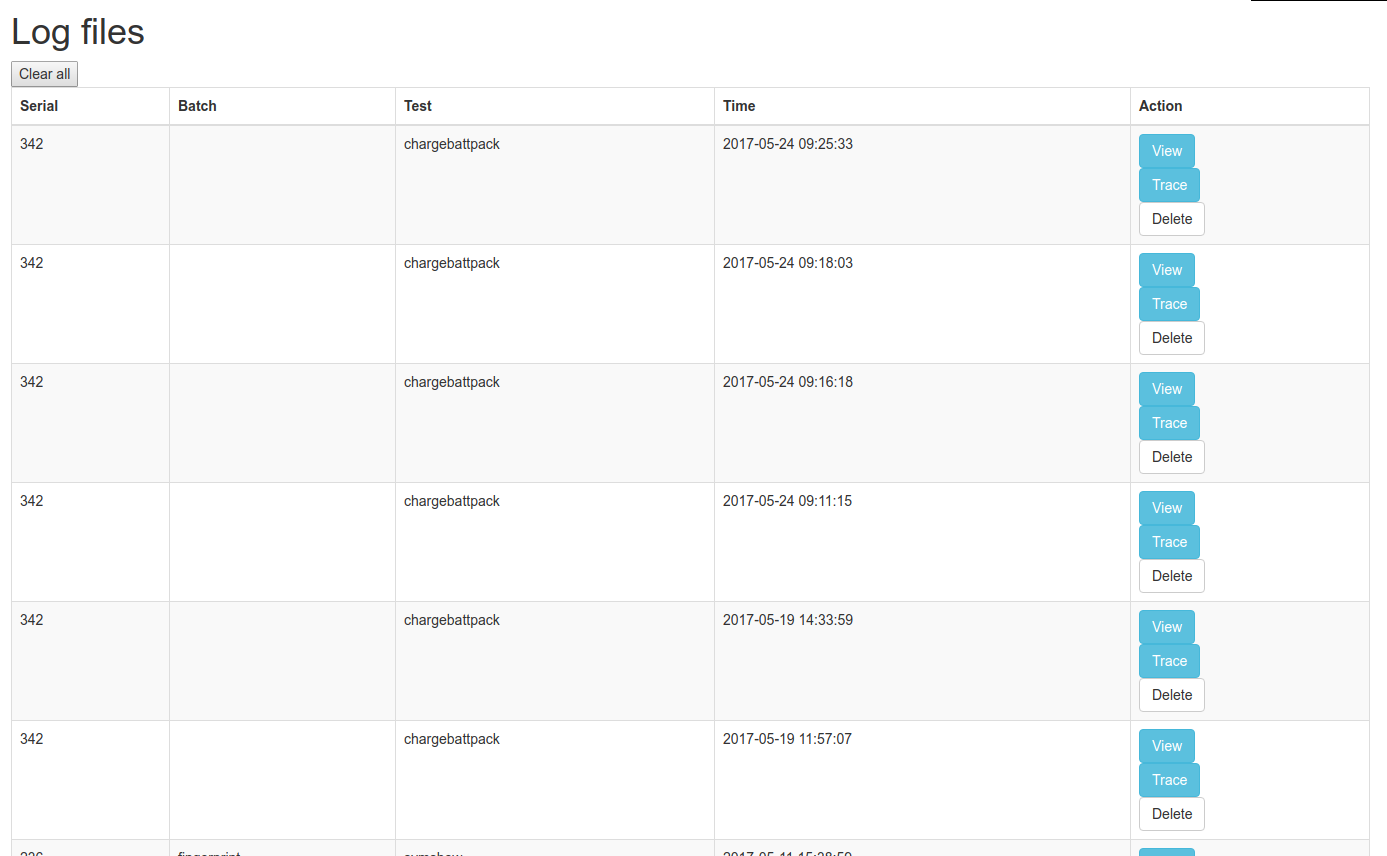
\includegraphics[scale=0.4]{wa_logs.png}
    \caption{The log page displaying all logs generated and some informations about them.}
    \label{wa_logs}
\end{figure}

\begin{figure}
    \centering
    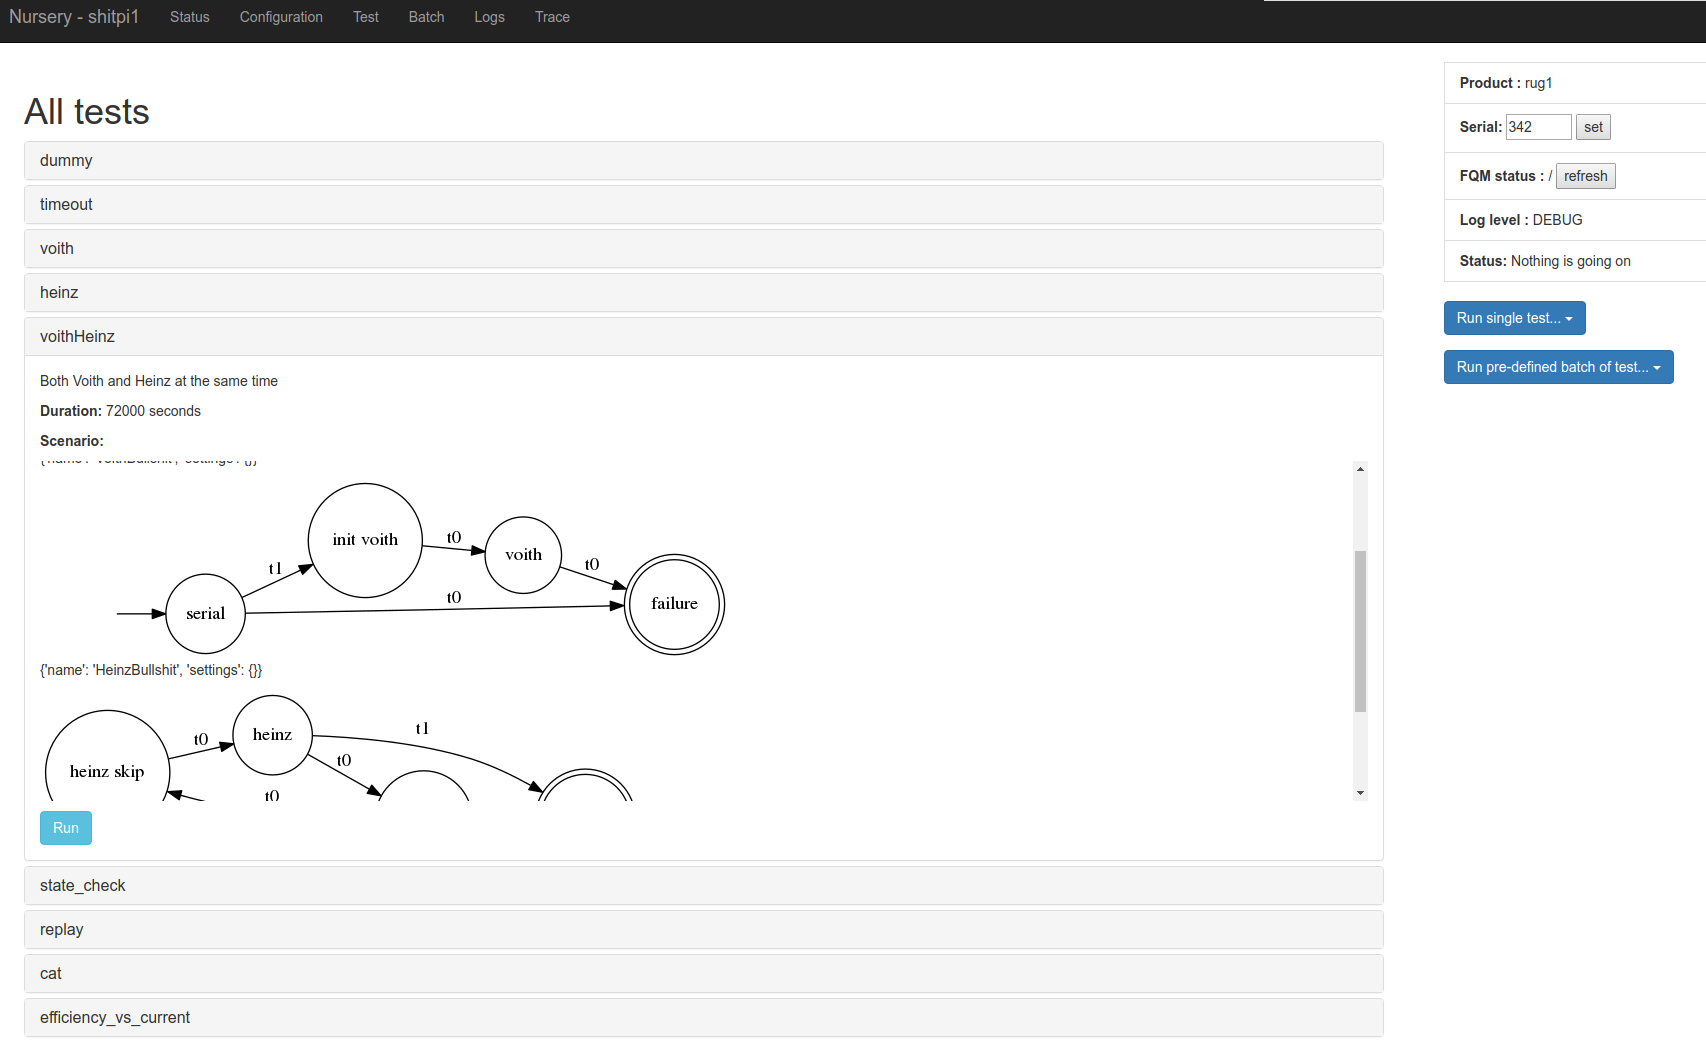
\includegraphics[scale=0.2]{wa_tests_doc.png}
    \caption{This page shows all the available documentation about each tests.}
    \label{wa_tests_doc}
\end{figure}

\begin{figure}
    \centering
    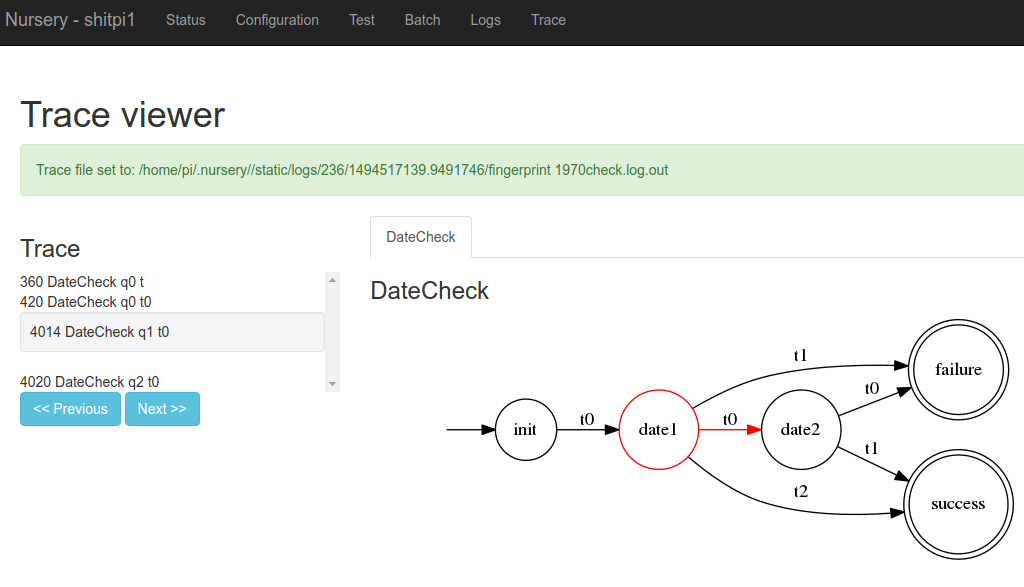
\includegraphics[scale=0.4]{wa_trace.png}
    \caption{here we can use a trace generated by Nursery to review the test execution.}
    \label{wa_trace}
\end{figure}


%------------------------------------------------------------------------%
%                                                                        %
%                                                                        %
% CONCLUSION                                                             %
%                                                                        %
%                                                                        %
%------------------------------------------------------------------------%

\clearpage
\part{Conclusion}

Putting the complexity as a limitation gave us a software that can run on any moder system. The simulation is hosted on RaspBerry Pi which are low end system. This allowed us to build a lot of Nursery system for a really cheap price, RaspBerry Pi costing around fifteen euros. We made around sixteen Nursery system separated into two areas. Height of them dedicated for RailsterOS verification and height of them used mainly for fingerprinting. So, using the work done in this thesis, we are now able to fingerprint the faulty RUG way faster. We need only one guy to analyze up to height of them in parallel using the Nursery systems we just talked about. The same thing hold true for RailsterOS testing. We can now leave newly developed version of it running on Nursery for days and get a report of all the errors that happened afterwards instead of waiting for errors to happen into the production environment. The total count of line of code in Python is about 7000 and 17 tests where developed with more to come.\\

My personal analysis lead me to think that the success of Nursery is based on the following key point:
\begin{itemize}
\item Will it be used by other users?
\item Will it save time or make life easier for some people?
\item Can we gain money from it?
\end{itemize}

Clearly, detecting fault earlier allows us to save money and time. No need to call back some hardware and less fault in production means less loss of money. We do not longer need to invest days of analyze for fingerprinting, all it takes is to plug the faulty RUG into Nursery and click a button. This could easily take up to 3 hours per RUG where now, we can do it in just one day of work for height RUG using more intensive testing cases! Lastly, some guys of the hardware team and from the supply chain were introduced with Nursery. We showed them how to write test for Nursery and they loved the way things were made and how simple it was. Their test were done in approximately one hour. This lead us to think that, with proper formations and documentation, other users could gladly uses Nursery.\\

I think that Nursery is a key assets that will become more and more used inside of Railnova. We even talked about using it for production lines in the future. But a lot of work is yet to be done on the accessibility aspect of it. Proper documentation needs to be written, some ideas are expected to ease a bit more the writing of tests like adding a generic state allowing us to create a transition from "any state" to one particular state without needing to repeat this transition to every other states and theres probably a lot more thing we didn't think about.

%------------------------------------------------------------------------%
%                                                                        %
%                                                                        %
%                                                                        %
%                                                                        %
%                                                                        %
%                                                                        %
%                                                                        %
%                                                                        %
%                                                                        %
% APPENDIX                                                               %
%                                                                        %
%                                                                        %
%                                                                        %
%                                                                        %
%                                                                        %
%                                                                        %
%                                                                        %
%                                                                        %
%                                                                        %
%------------------------------------------------------------------------%

\appendix

%------------------------------------------------------------------------%
%                                                                        %
%                                                                        %
% IO ABSTRACT                                                            %
%                                                                        %
%                                                                        %
%------------------------------------------------------------------------%

\clearpage
\section{Abstraction of Inputs/Outputs}

This part of the work is dedicated on describing how we managed to write simple piece of software that assure the link between Nursery and the real world/\gls{rug}.

% \subsection{About Inputs/Outputs}

% As we are working with a system that we feed with inputs and as we are ourselves feeded by the system's outputs, the concept of \gls{io} is a bit confusing. On the figure~\ref{io_abstract}, you can visually see why it is ambiguous. So at this point, we'll simply consider that when we talk about inputs, we mean inputs of the system and when we talk about outputs, we talk of what the system produce.\\

% \begin{figure}
%     \centering
%     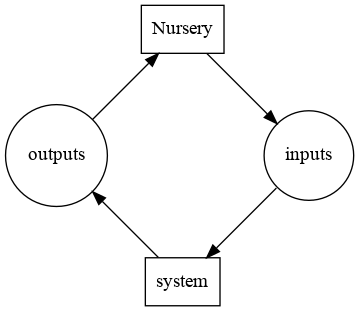
\includegraphics[scale=0.6]{io_abstract.png}
%     \caption{Inputs of the system are outputs of Nursery and vice/versa}
%     \label{io_abstract}
% \end{figure}

\subsection{Outputs}

Let us start with the outputs. By outputs we mean all the data produced by the \gls{rug} or, more generally speaking, all data produced by the reviewed system. Those have been abstracted with a layer of object called output providers. Their goal is to retrieve outputs from various places and feed them into Nursery as they go.\\

For example, we can imagine that we want to receive some data each time the system sends data to a server, each time the system produce a sound, etc. All of this is possible as we simply need to write a script that detects that and use some kind of API to feed them through Nursery.\\

\subsubsection{How does it works}

So, internally, each output provider defines a type of data it provides. For example, lets say we want to send data to nursery each time someone put a message on Twitter, we could name our data type: "TWITTER". Then, each test that is interested in data of type "TWITTER" will be subscribed to our output provider. It also allows us to ignore output providers for which no test are interested in. Practically speaking, the only output providers running for a given test will be those that provide a data type useful for the test.\\

Our provider is bundled with a mean of communication with all scenario that are subscribed to the data type it provide. With it, we can send data to every listener with one simple call. All the communication process is managed internally in Nursery.
In our provider, we have a function that allows us to broadcast data to all listener. With this approach, we can write output providers for any type of data we can think of, all we have to do is defining the data type we provide and which output provider provides it in a configuration file and then implement this output provider, that's it, now any scenario can listen to this particular data type.\\

One limitation though is that every data type can be produced by at most one output provider. On the other hand, every output provider can produce as much data type we want if this becomes a requirement at some point.\\

\subsubsection{Wanesy}

The first data type we have develop is the WANESY data type. Data of type WANESY are triggered when we receive a new pack of data sent by \gls{railsteros} to our server online. The method to retrieve them is simply to poll a JSON generated list of message by HTTP and check timestamp of generated messages, when a newer timestamp appears, we get the message and send it into Nursery.\\

Another more effective way of doing this would be by direct connection to the database but this would probably introduce security issues and is not really required for our use case. Note that it is still feasible in future version of this work.

\subsubsection{Log}
\label{subsec:log}

This data type is more of Grey-Box testing as it requires a direct serial connection into the studied system so we assume that we  are working on some kind of \gls{rug} and that we know where the log are located on it. Nevertheless, this data type ("LOG") is useful to provide more complex information wen fault arise and also help us to design more intrusive tests.\\

So even if they are a bit out of scope here, they do not invalidate the fact that our system can work on Black-Box testing.\\

To design those test, as we previously stated, we simply initiate a serial connection over the \gls{rug} and then download the file located in the log folder. Then, our script process it and send new lines into Nursery.

\subsubsection{Miscellaneous}
\label{subsec:misc}

As we talked in sub-section ~\ref{subsec:log}, we can initiate a serial communication with the \gls{rug}. Using this serial communication, we can send command to it in an Unix environment so it's easy for us to check a lot of properties for our tests needs. Of course, this is clearly white-box testing, we know how the system is supposed to work so we can ask it if some key file are in place, if all environment variables seems to be correct, do some statistics on some values to be sure they have correct values all along our tests and things like that.\\

\subsection{Inputs}

Some of our test make use of external devices to produces inputs that are feeded to the \gls{rug} or to the hardware being tested. Those devices are, for example, a power module that can charge the battery of our \gls{rug}, thermic chamber that can manipulate the current temperature to stress test our hardware in extreme conditions and things like that.\\

We also have more direct inputs like the Ethernet connection, we want to be able to disconnect or re-connect the tested process or hardware.

\subsubsection{Power Management}

\begin{figure}
    \centering
    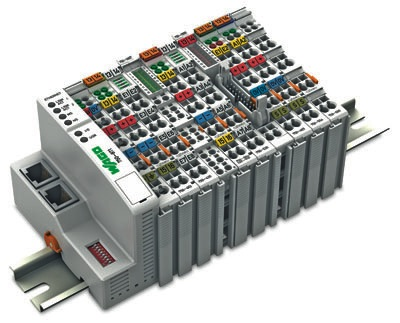
\includegraphics[scale=0.6]{wago_module}
    \caption{Module used to manage the power status of a \gls{rug}}
    \label{wago}
\end{figure}

To control the power status, we need to send a command to a Wago module like the one of the figure~\ref{wago}. Those modules are connected via an Ethernet connection thus we need to open a TCP port to communicate with it and then send a command to select which power supply we want to control and what we want to do (power on or power off).

\subsubsection{Connectivity}

Controlling the connectivity is not something we did but this is easily done by using some advanced switch. We simply need to communicate with it and send commands to deactivate the Ethernet port to which the \gls{rug} is connected.

\subsection{The generic way}

Some techniques we mentioned, like in sub-section ~\ref{subsec:log} and sub-section ~\ref{subsec:misc}, use some kind of white-box testing. As one could expect, those techniques can only be used for one given device. We cannot initiate a serial connection with every process or hardware we want and all of them don't have the same Unix environment to dialog with.\\

But even the ones that applies to black-box testing can only be specific to some restraint set of process or hardware. Here, our techniques are all specific for \gls{rug} hardware. So every time we need to test a new kind of process or hardware, we will need to write some code to retrieve outputs and provides inputs for it. That's what we kept in mind all along this project by designing what we called \gls{op}.\\

\subsubsection{Outputs}

\gls{op} were designed to provides asynchronous capabilities to our tests. Polling \gls{io} is a process that takes a lot of times compared to the execution time of our test. With \gls{op}, we get the data when they are ready and we don't have to wait for them by freezing all the test. Two ways of retrieving data were implemented.\\

The most trivial way is simply to send data periodically to all test that needs it. The test knows he will receive data but he does not knows when. The test must be designed accordingly. This is useful to fetch data that are not fixed like a speed, the current time or the remaining fuel for example.\\

The second way is to ask for data from the test. The call is asynchronous so you simply notify the \gls{op} that you are ready to receive some data or that you want it to fetch some data right now. This allows us to ask for one-time data like a serial number or other kind of data that are not supposed to change depending on the time.\\

So the first method is more for data you want to be able to monitor and the second method is more for data you will only need once.\\

\subsubsection{Inputs}

For inputs, we simply need some software to which we can send commands so we don't need so much abstraction as for the outputs. We are not in an asynchronous system. The way to go we adopted was simply to develop some software that accepts command and send inputs to whatever we want.\\

One example was a software we used that can control a thermionic chamber. With it, we were able to control the temperature in which our \gls{rug} was evolving. And of course, we can use it for other systems too, and we did it to test other pieces of hardware.

Another example, more specific, was a software used to control a device that could apply different electric loads to any device we connected with it. This was useful for some hardware test that had nothing to do with the \gls{rug}.


%------------------------------------------------------------------------%
%                                                                        %
%                                                                        %
% TEST CASES                                                             %
%                                                                        %
%                                                                        %
%------------------------------------------------------------------------%

\clearpage
\section{Test cases}

Here we will give explanation and details on some practical cases we had to deal with.


\subsection{Timeout check}
%-----------------------------------------------------------------------------

This test was designed to make sure that the \gls{rug} is sending informations to our servers. To do that, we need an \gls{op} that will fetch all messages received from the studied \gls{rug} and fetch them to our \gls{fsm}. Our \gls{fsm} will then check that data are received at least every 30 seconds.\\

\begin{figure}
    \centering
    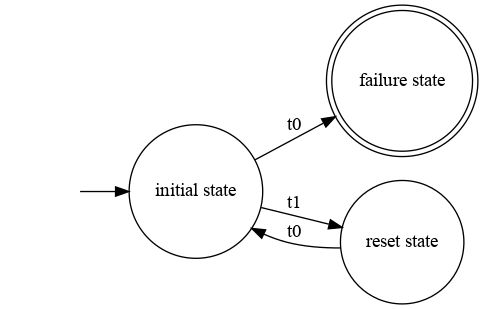
\includegraphics[scale=0.6]{graph/TimeoutCheck}
    \caption{\gls{fsm} for the timeout check}
    \label{timeoutcheck}
\end{figure}

The figure~\ref{timeoutcheck} shows how we designed this test. Transition are, of course, complex so we only show a simplified name for them. They are quite obvious given the rest of the diagram.


\subsection{Date check}
%-----------------------------------------------------------------------------

This test verify that the system uses the correct date. With an incorrect date set, the messages sent by it to the Railnova servers will be discarded resulting in a loss of communication from this device.\\

This test uses the serial connection and make uses of Unix commands directly on the system thus this is not a black-box testing processes.\\

The most complicated part here is to get the serial connection, a lot of troubles can arise while trying to log-in the system. Once we have a valid serial connection, we can simply issue a "date" command and parse the result. The date is updated through GPS/GSM antenna communication and this process can take up to an hour so if the date is not set right (if the date appears to be in 1970), we simply wait an hour and then, issue the test again.\\

1970 is the date you get when the timestamp is not set. This is because of how Unix and timestamp systems works.

\begin{figure}
    \centering
    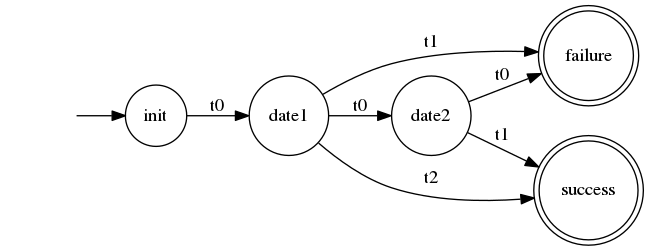
\includegraphics[scale=0.6]{graph/DateCheck}
    \caption{\gls{fsm} for the date check}
    \label{datecheck}
\end{figure}


\subsection{Battery cycle}
%-----------------------------------------------------------------------------

We made some test that where not related to the \gls{rug}. One of those was able to charge a battery and then discharge it. The goal of this was measure the electrical levels all along those steps to determine whether or not the battery is working.\\

As shown in the figure~\ref{battcycle2}, we made several cycle of charge/discharge. This particular test was designed for a piece of hardware and not for a software. This is a sufficient proof to show that our system work as well for a software than it does for hardware.

\begin{figure}
    \centering
    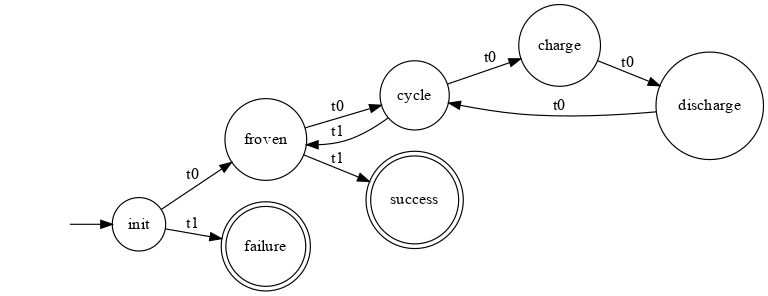
\includegraphics[scale=0.4]{graph/BatteryCycle.png}
    \caption{\gls{fsm} for the battery cycle}
    \label{battcycle2}
\end{figure}

\clearpage
\addcontentsline{toc}{section}{References}
\bibliographystyle{IEEEtran}
\bibliography{ref}{}

\clearpage
\printglossaries


\includepdf[pages={3}]{template.pdf}

\end{document}
